% arara: xelatex: {shell: true}
% arara: biber
% arara: makeglossaries
% arara: xelatex: {shell: true}
% arara: xelatex: {shell: true}
\documentclass[letterpaper,11pt]{article}
\usepackage[margin=1in]{geometry}
\usepackage{newfloat}
\usepackage{hyperref}
\usepackage{graphicx}
%\usepackage[justification=centering,font=small,labelfont=bf]{caption}
\usepackage[font=small,labelfont=bf]{caption}
\usepackage{fancyhdr}
\usepackage{parskip}
\usepackage[section]{placeins}
\usepackage{epigraph}
\usepackage{sourcecodepro}
\usepackage{fontspec}
\usepackage[toc,nonumberlist,xindy]{glossaries}
\usepackage{relsize}
\setmonofont[Scale=0.7]{Source Code Pro}
\defaultfontfeatures{Ligatures=TeX}
\usepackage{xcolor}
\usepackage[titletoc,title]{appendix}
\usepackage{minted}
\usepackage{csquotes}
\usepackage{polyglossia}
\setmainlanguage{english}
\setotherlanguage{hebrew}
\setotherlanguage{french}
\newfontfamily\hebrewfont[Scale=0.8,Script=Hebrew]{Frank Ruehl CLM}
\definecolor{dsscawpurp}{HTML}{b079b0}
\definecolor{dsscawpurpcap}{HTML}{6c286c}
\usepackage[font={color=dsscawpurpcap},labelfont={sc}]{caption}
\usepackage[backend=biber,
date=iso,
seconds=true,
style=numeric,
bibencoding=utf8,
]{biblatex}

\addbibresource{\jobname.bib}
\usemintedstyle{friendly}
\newenvironment{denseitemize}{
  \begin{itemize}
      \setlength{\itemsep}{0pt}
}{
  \end{itemize}
}
% An attractive 'C++'
\newcommand\CC{C\nolinebreak\hspace{-.05em}\raisebox{.4ex}{\relsize{-3}{\textbf{+}}}\nolinebreak\hspace{-.10em}\raisebox{.4ex}{\relsize{-3}{\textbf{+}}}\hspace{.2em}}

\pagestyle{fancy}
\rhead{
  
\includegraphics[height=\fontcharht\font`\D,keepaspectratio=true]{../dsscaw-hdr.pdf}
  \textcolor{dsscawpurp}{DSSCAW Technical Report \#004}
}

\title{Hacking the Planet! with Notcurses:\\
A Guide to TUIs and Character Graphics\thanks{
 \href{https://www.dsscaw.com/}{Dirty South Supercomputing of Atlanta, GA. Free documentation under the Apache 2.0 License.}
}\\
}
\author{Nick Black, Consulting Scientist\\
\texttt{nickblack@linux.com}
}

\makeglossaries
\setglossarypreamble{When possible, I have followed the definitions of
  RFC 2978\cite{rfc2978} and the Glossary of Unicode Terms\cite{unicodeglossary}.}
\loadglsentries{glossary}

%%%%%%%%%%%%%%%%%%%%%%%%%%%%%%%%%%%%%%%%%%%%%%%%%%%%%%%%%%%%%%%%%%%%%%%%
\begin{document}
%%%%%%%%%%%%%%%%%%%%%%%%%%%%%%%%%%%%%%%%%%%%%%%%%%%%%%%%%%%%%%%%%%%%%%%%
%\date{Feb 14, 2020}
\maketitle
%\thispagestyle{fancy}
\date{}
\vspace{1in}
\begin{center}
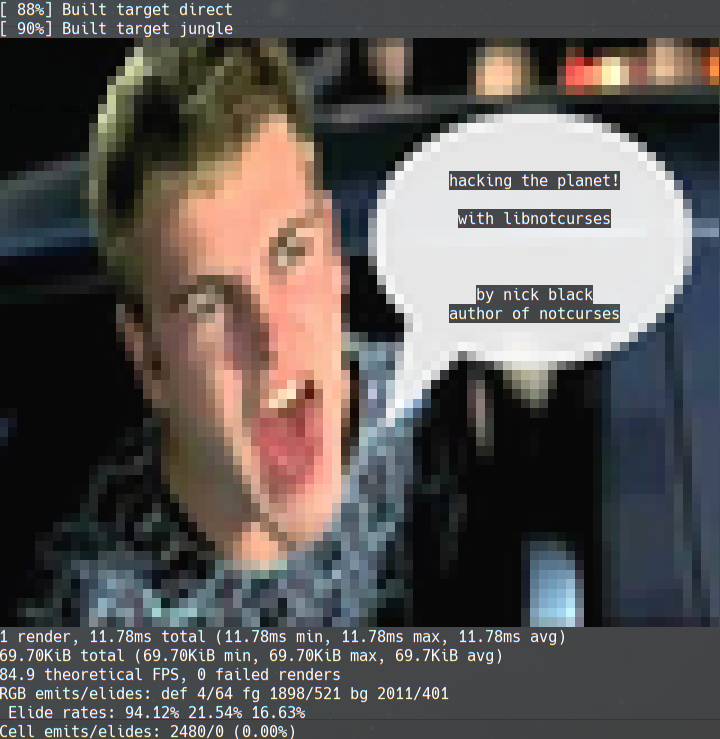
\includegraphics[width=.75\linewidth]{htp-with-notcurses.png}
\end{center}
\thispagestyle{empty}
%%%%%%%%%%%%%%%%%%%%%%%%%%%%%%%%%%%%%%%%%%%%%%%%%%%%%%%%%%%%%%%%%%%%%%%%

\clearpage
\pagenumbering{roman}

\vspace*{1in}
\begin{center}
  \textit{For T.\ S.\ Eliot, il miglior fabbro.} \\
  \vspace{.25in}
  \textit{For Jim Greenlee, for speaking rigor to my programming.\\
  \vspace{.25in}
  For Coach Jeanette Martin, for exhortations to go H.A.M. \\
  \vspace{.25in}
    For Professor Hyesoon Kim, for introducing me to the glorious world
    inside the die.\\
  \vspace{.25in}
    For Professor Richard Vuduc, who
    demonstrates serenity in brilliance, and kindness in dominance.\\}

  \vspace{1in}\ldots but mostly for Emily.
\end{center}
\clearpage
%%%%%%%%%%%%%%%%%%%%%%%%%%%%%%%%%%%%%%%%%%%%%%%%%%%%%%%%%%%%%%%%%%%%%%%%

\tableofcontents

\cleardoublepage
\phantomsection
\addcontentsline{toc}{section}{\listfigurename}
\listoffigures
\listoflistings
\listoftables
\clearpage
%%%%%%%%%%%%%%%%%%%%%%%%%%%%%%%%%%%%%%%%%%%%%%%%%%%%%%%%%%%%%%%%%%%%%%%%

\newpage

\vspace*{1.25in}
\begin{figure}[!htbp]
\centering
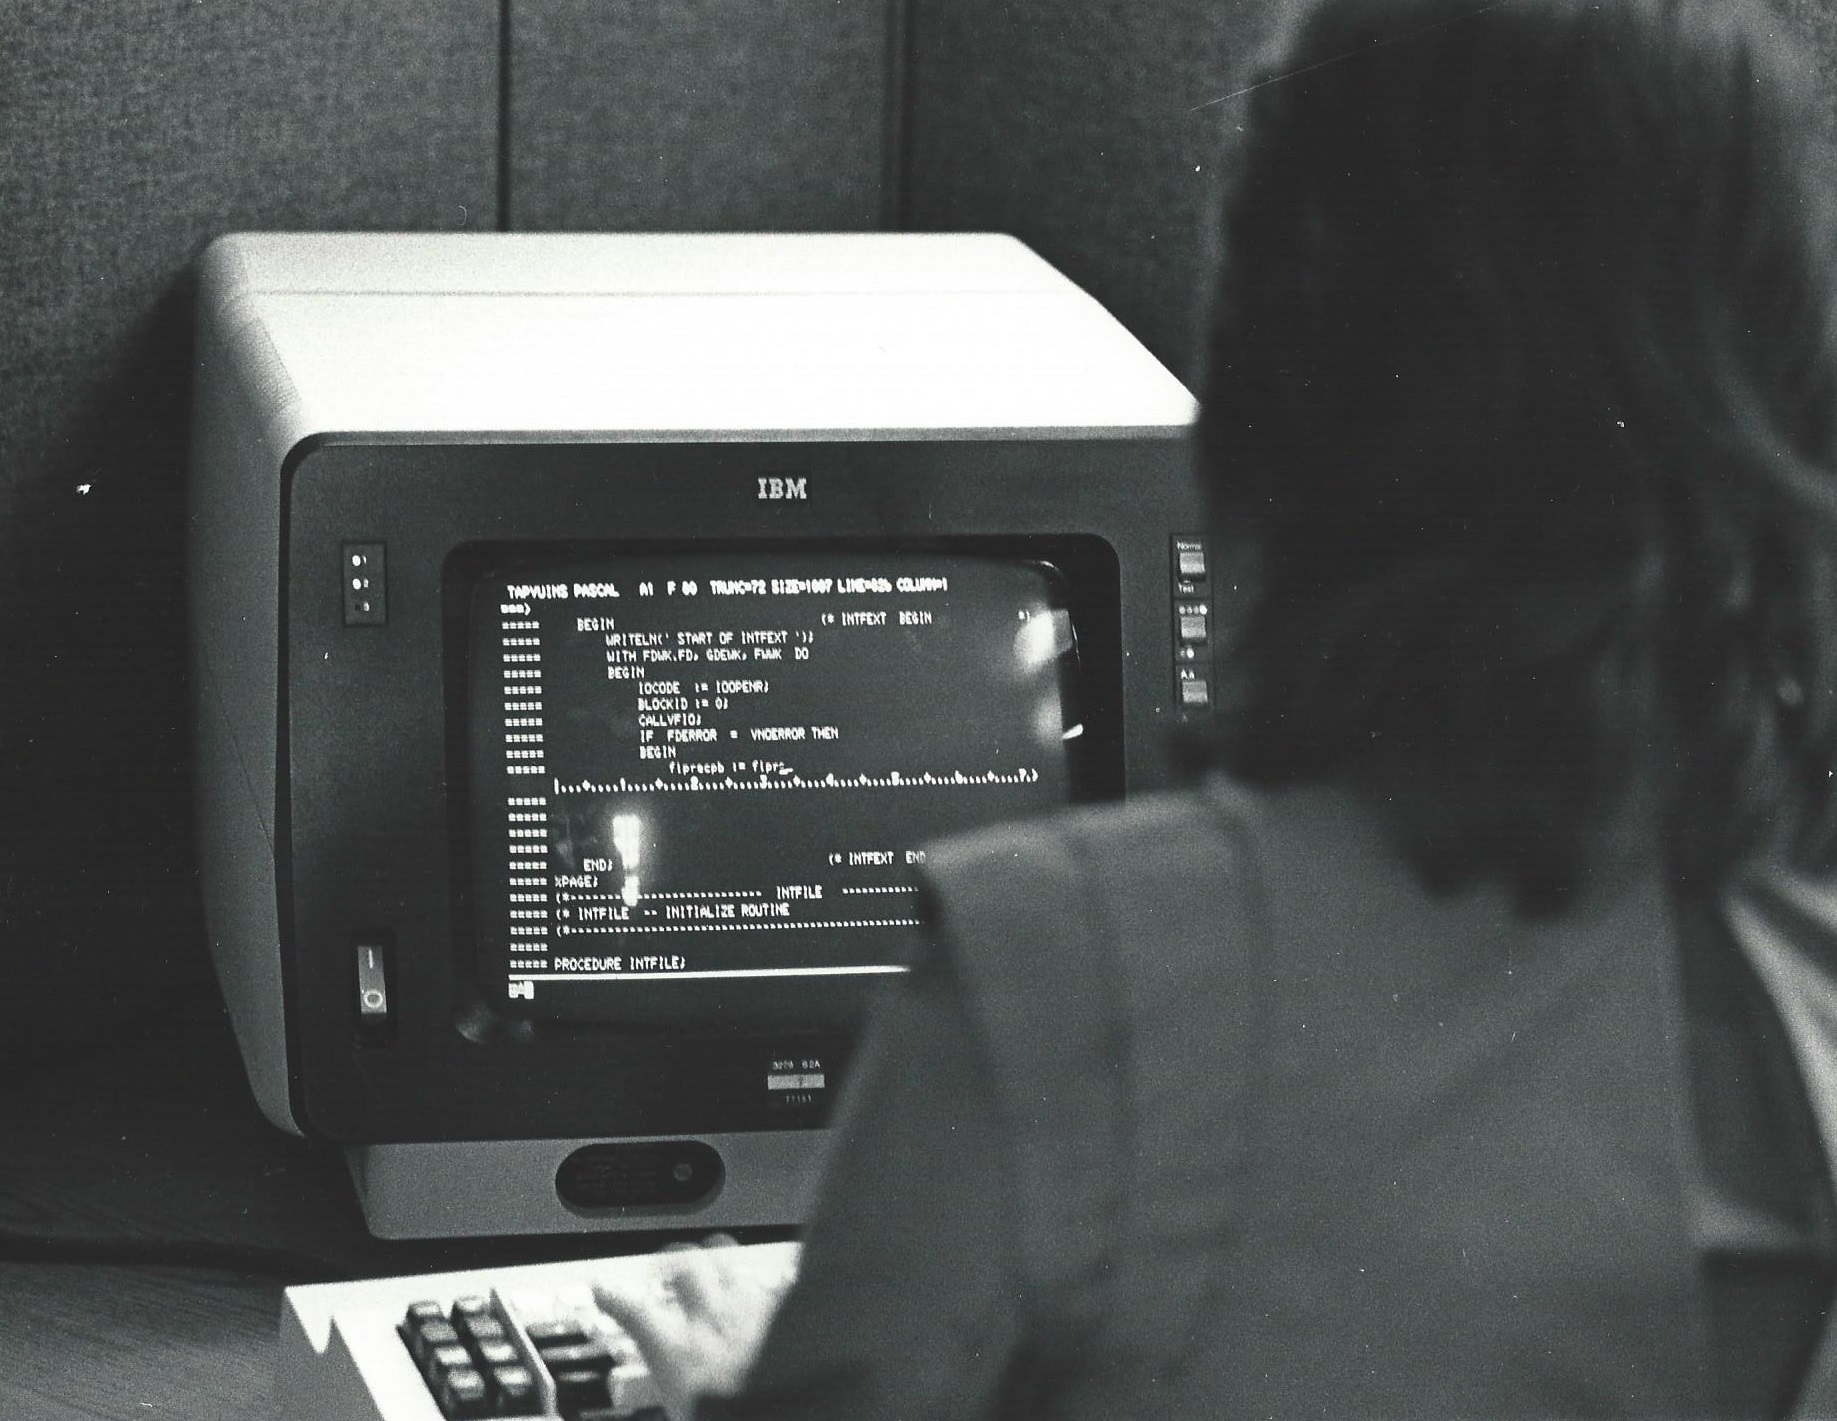
\includegraphics[width=1\linewidth]{media/ibm3270.jpg}
\caption[A programmer at her IBM 3270]{A programmer at her IBM 3270 2A. \textit{Source: Jonathan Schilling}.}
\end{figure}
\clearpage
%%%%%%%%%%%%%%%%%%%%%%%%%%%%%%%%%%%%%%%%%%%%%%%%%%%%%%%%%%%%%%%%%%%%%%%%
\vspace*{1in}
\section{Foreward}
Copyright © 2020 Nick Black.

\small{This edition corresponds to version 1.2.2 of the Notcurses
library, released 2020-02-24.

Notcurses can be downloaded from
\url{https://github.com/dankamongmen/notcurses}.

This document can be downloaded
from~\url{https://nick-black.com/htp-notcurses.pdf}.

Licensed under the Apache License, Version 2.0 (the ``License''); you may not use
this file except in compliance with the License. You may obtain a copy of the
License at \url{http://www.apache.org/licenses/LICENSE-2.0}.

Unless required by applicable law or agreed to in writing, software
distributed under the License is distributed on an ``AS IS'' BASIS,
WITHOUT WARRANTIES OR CONDITIONS OF ANY KIND, either express or implied.
See the License for the specific language governing permissions and
limitations under the License.

Tetris © The Tetris Company, LLC.
\textit{Hackers (1995)} © United Artists Pictures.
\textit{House of Leaves (2000)} © Penguin Random House.
``Ruins with Rain'' © Mark Ferrari/Living Worlds.
``Final Fantasy'' © Square Enix Co Ltd.
``Super Mario Bros.'' © Nintendo of America.
``Ninja Gaiden'' © Koei Tecmo America.
``Street Fighter II'' and ``Mega Man 2'' © Capcom of America.

\vspace*{1in}
\subsection{¡Peligro!}

The code written for this book attempts to minimize use of vertical space
without eliding error checking (or crossing into the realms of the grotesque).
Error handling is a fundamental slog of C programming, one that
inevitably complicates reliable applications.

\textbf{These listings cannot be considered examples of good general style\ldots but they \textit{do} get the job done.}

}


\vfill

\begin{center}
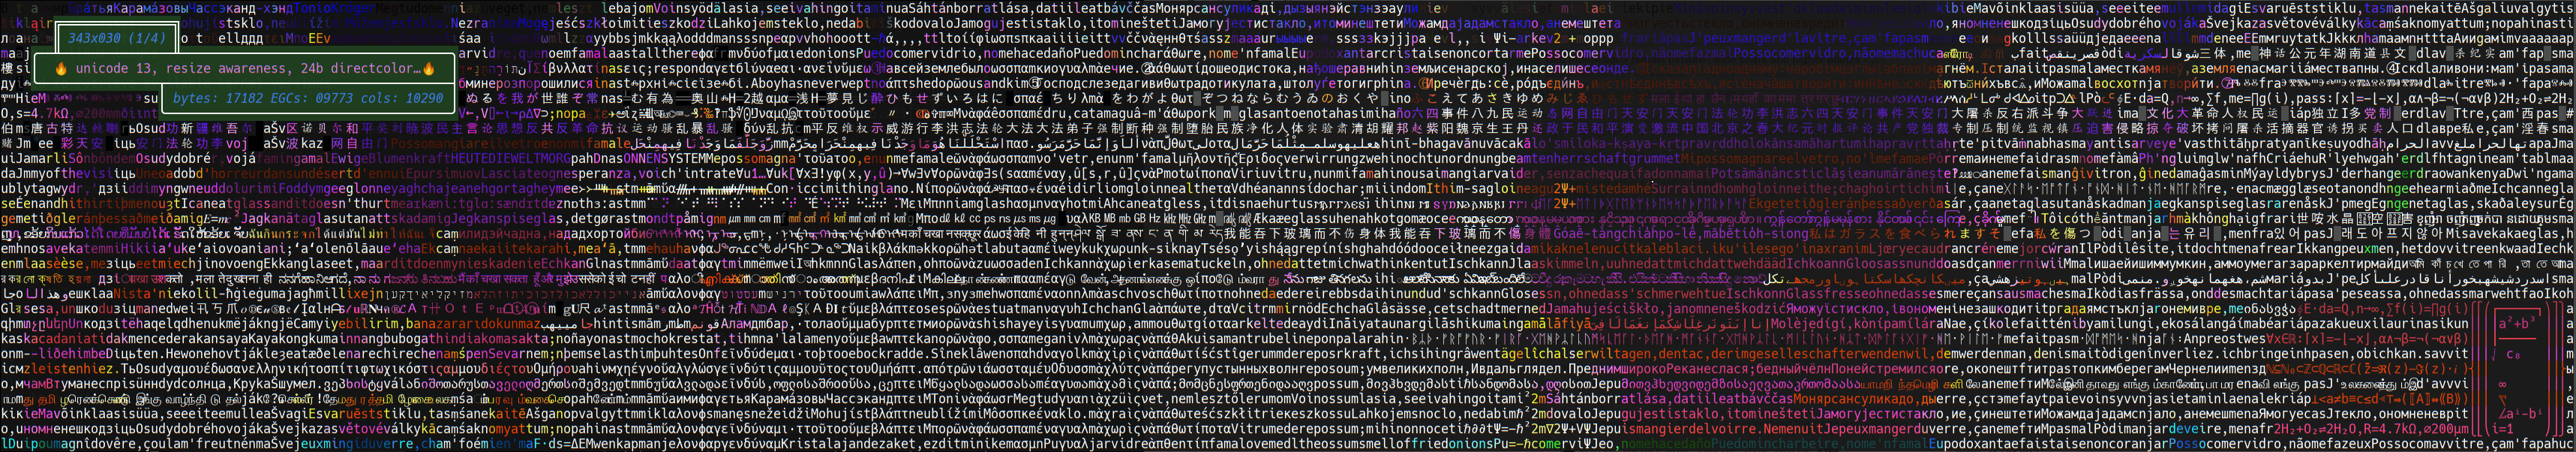
\includegraphics[width=1\linewidth]{media/widechars.png}
\end{center}

\clearpage
%%%%%%%%%%%%%%%%%%%%%%%%%%%%%%%%%%%%%%%%%%%%%%%%%%%%%%%%%%%%%%%%%%%%%%%%
\pagenumbering{arabic}

\epigraph{Our fine arts were developed, their types and uses were established, in times
very different from the present, by men whose power of action upon things was
insignificant in comparison with ours. But the amazing growth of our
techniques, the adaptability and precision they have attained, the ideas and
habits they are creating, make it a certainty that profound changes are
impending in the ancient craft of the Beautiful.}{Paul Valéry}
\section{Introduction}

I implemented Notcurses in the winter of 2019 after having a few patches
rejected from NCURSES. The first commit was pushed 2019-11-16. I started
writing this manuscript 2020-02-12, following the 1.1.8 release. It proved to
be seductive as hell, and it was only with difficulty that I tore myself away
following three months of hard work. By that time, Notcurses subsumed large
chunks of NCURSES, adding a great deal more. The project had three
major goals:

\begin{denseitemize}
\item to provide NCURSES-like functionality with 24-bit color, safety in the
    presence of multithreading, and full Unicode support,
\item to reduce the amount of boilerplate code necessary for the UIs of my
    TUI applications, including \textit{growlight} and \textit{omphalos}, and
\item to portably facilitate the most vivid character graphics possible.
\end{denseitemize}

Many people asked how such a thing was useful. My usual response was that
numerous devices don't present a bitmap interface, that X11 GUIs run remotely
over SSH are effectively unusable, that plenty of machines don't have a GUI
environment installed, that there are obvious applications for large outdoor
displays, and that Sixel isn't well-supported across different
terminal emulators. It seems impossible in an age of gigatransistor graphics
cards, but the text environment still presents perceivably less latency
than most GUI toolkits. That I was able to remove thousands of lines
of NCURSES code from my applications was a nice side benefit.

In truth, the main reasons were that it was fun, and I wanted to see how far
I could push it.

As I write this, Notcurses is present in Arch's AUR, and is awaiting promotion
from the Debian Incoming queue. Written as a C core, it enjoys \CC, Python, and
Rust wrappers. I have submitted it as a backend to NEStopia and RetroArch, and
intend to integrate it into Mesa as an OpenGL backend. So long as one can live
with the limited resolution available when a screen is divided into rectangular
cells, it can handle any graphics thrown at it. I hope to see it displace
NCURSES as the go-to character graphics library for new applications (there is
little value in porting existing applications to Notcurses, since an unchanged
application wouldn't take advantage of its advanced features).

While the X/Open Curses specification is unlikely to ever go away (nor should
it, as a lowest-common-denominator interface to devices Notcurses is unlikely
to ever support), I believe Notcurses to present a superior API and
implementation for modern TUI applications.

The console ain't dead! Hack on, hax0rs.

\vfill

\begin{flushright}
  \textit{---February 2020, Atlanta}
\end{flushright}

\newpage
%%%%%%%%%%%%%%%%%%%%%%%%%%%%%%%%%%%%%%%%%%%%%%%%%%%%%%%%%%%%%%%%%%%%%%%%

\vfill
\begin{center}
%
\includegraphics[width=.4\linewidth]{../common/dsscaw-purp-scaled.png}
%
\includegraphics[width=.5\linewidth]{../common/south.png}
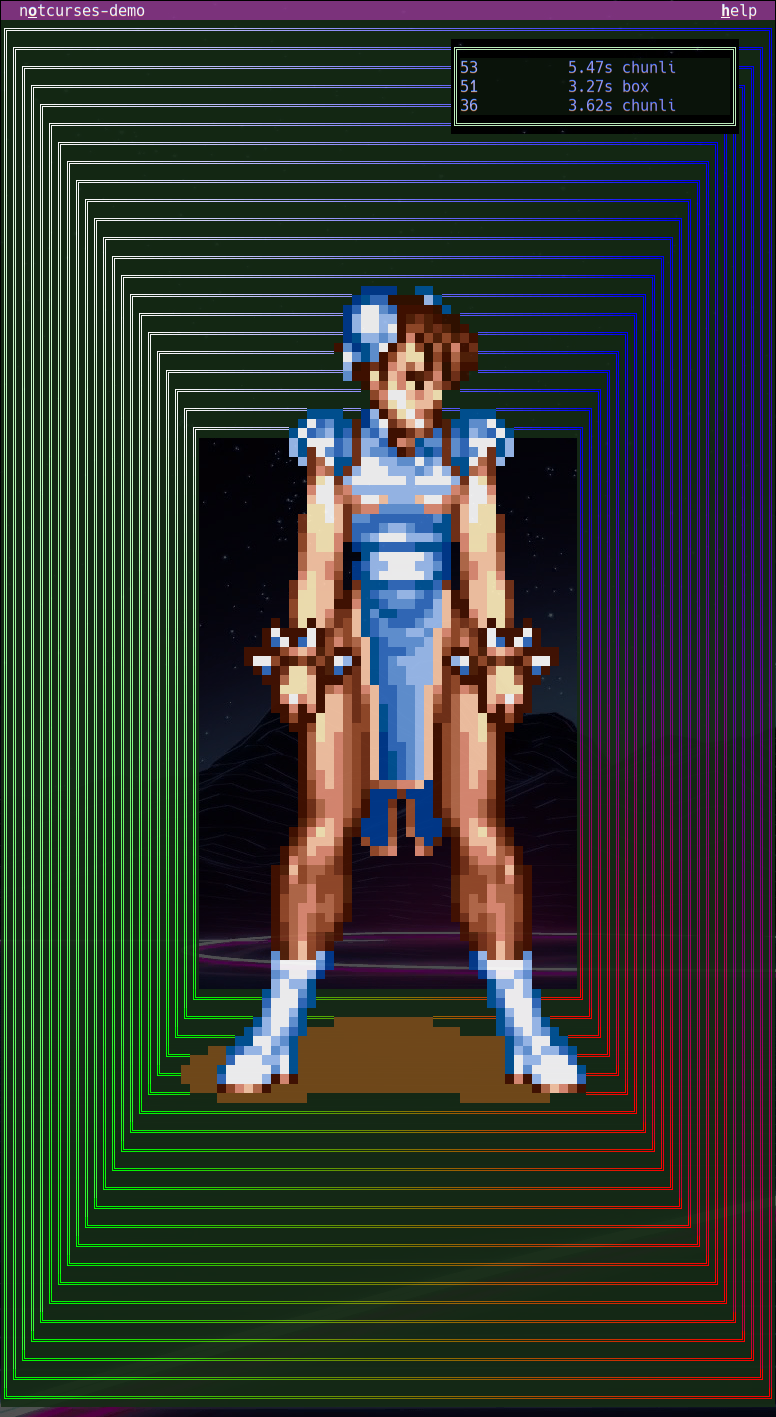
\includegraphics[width=.75\linewidth]{media/chunli-box-front.png}
\end{center}
\vfill
\section{Right, what's all this, then?}
Character graphics, aka text mode, aka the display side of a terminal, is
visualization that works with fonts rather than a pixel framebuffer\footnote{``Contones'', as raster graphics are known to printers.}
or a vector canvas\footnote{Nothing keeps you from implementing character graphics
with pixels or vectors, of course.}. There is furthermore an expectation that
this font is a fixed-width one---that all rendered glyphs are integer multiples
of some narrowest non-trivial glyph.

Given the same display hardware,

\begin{denseitemize}
\item{Character graphics are usually strictly less powerful than pure raster graphics, and}
\item{their lower effective resolution typically implies lower bandwidth requirements.}
\end{denseitemize}

A TUI (text user interface) is a holistic model, view, and controller implemented
using character graphics. TUIs, like WIMP\footnote{Windows, icons, menus, pointers, a paradigm so pervasive that
the industry collectively treasures a Wiemarian memory of Xerox PARC's noble
engineers stabbed in the back by management (not unlike the Oatmeal-fostered\cite{fuckoatmeal}
myopia regarding Edison and Tesla. I'll take Thomas Alva over Matthew Inman any
day). It too often goes unmentioned that the Alto and Star were as unusable as they were visionary\cite{lightningdealers}.
This is of course still superior to Java, which isn't even visionary.} GUIs,
freely move the cursor around their rectilinear display, as opposed to
line-oriented CLIs and their ineluctable marches through the scrolling region.

Given the same interactive task\footnote{These relations are not
fundamental, but emerge from the grim meathook realities of GUI toolkits.}

\begin{denseitemize}
\item{A TUI implementation is almost certainly a smaller memory and disk footprint than a GUI,}
\item{a good TUI implementation might introduce less latency, and}
\item{a properly-done TUI implementation can often be significantly more portable.}
\end{denseitemize}

Of course, it can also be a big pile of character graphics shit.

For over two decades, NCURSES (a free software implementation of the X/Open Curses\cite{cursesosi}
specification, plus extensions\cite{ncursesfaq}) has been a ubiquitous go-to for implementing
TUIs. Its maintainter (and author, in large part), Thomas E.\ Dickey,
exemplifies conservative and fastidious stewardship. Perfectly lovely TUIs can
be built using NCURSES, as seen in Figure~\ref{fig:ncurses-tuis}, but it \textit{does}
have its origins in the 8-bit era, and is showing its age.

\begin{figure}[!hbtp]
  \centering
    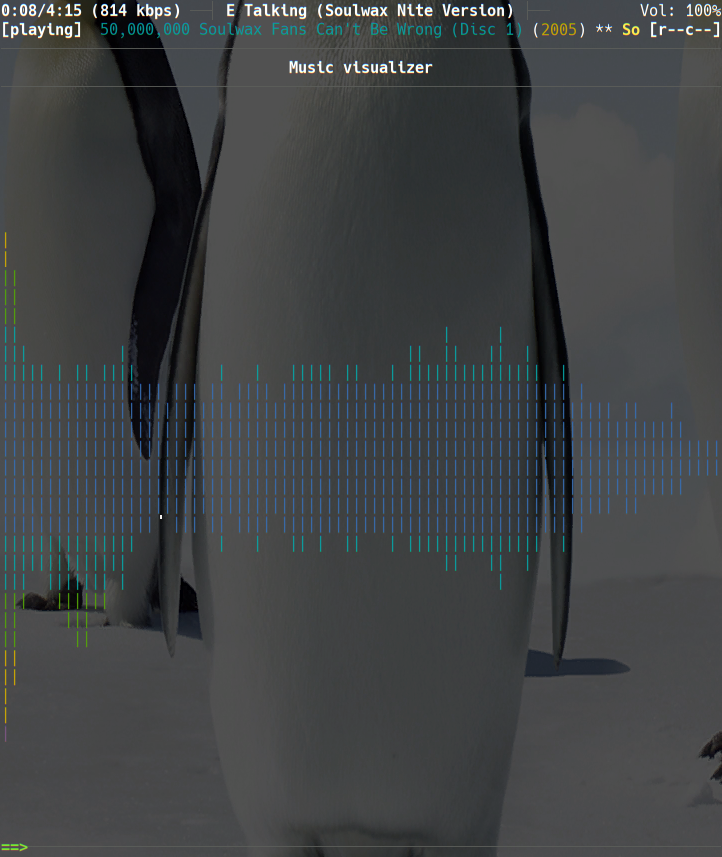
\includegraphics[width=.4\linewidth]{media/tui-ncmpcpp.png}
    \hfill
    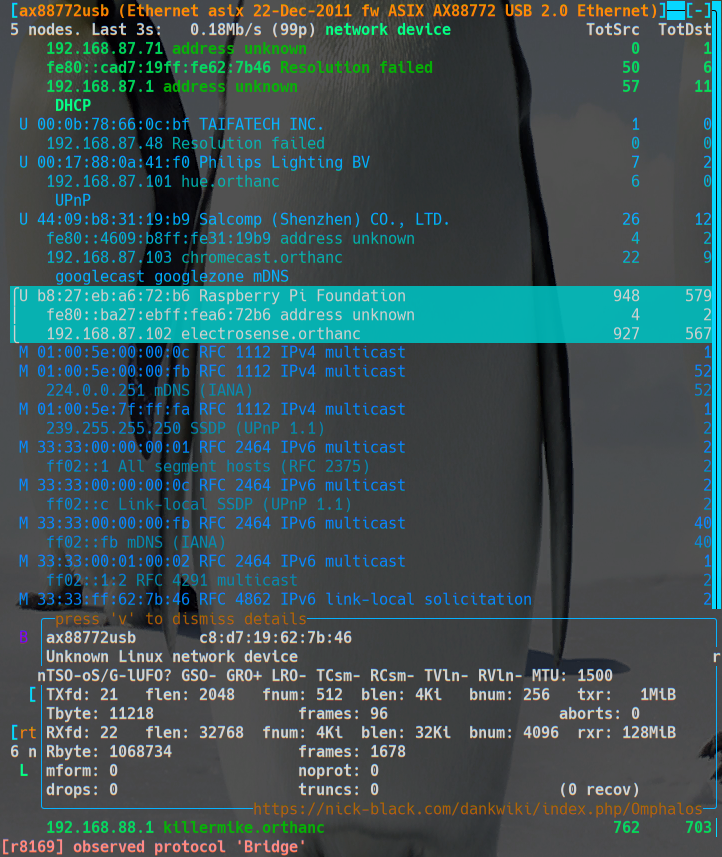
\includegraphics[width=.4\linewidth]{media/tui-omphalos.png}
    \caption[NCURSES TUIs: Ncmpcpp and Omphalos.]
    {\texttt{ncmpcpp}, a \CC application
      that has driven my Music Player Daemon since 2008 or so.
      \texttt{omphalos}, a C application
      written using NCURSES in its extended mode.}
  \label{fig:ncurses-tuis}
\end{figure}

\begin{figure}[!htbp] \centering
    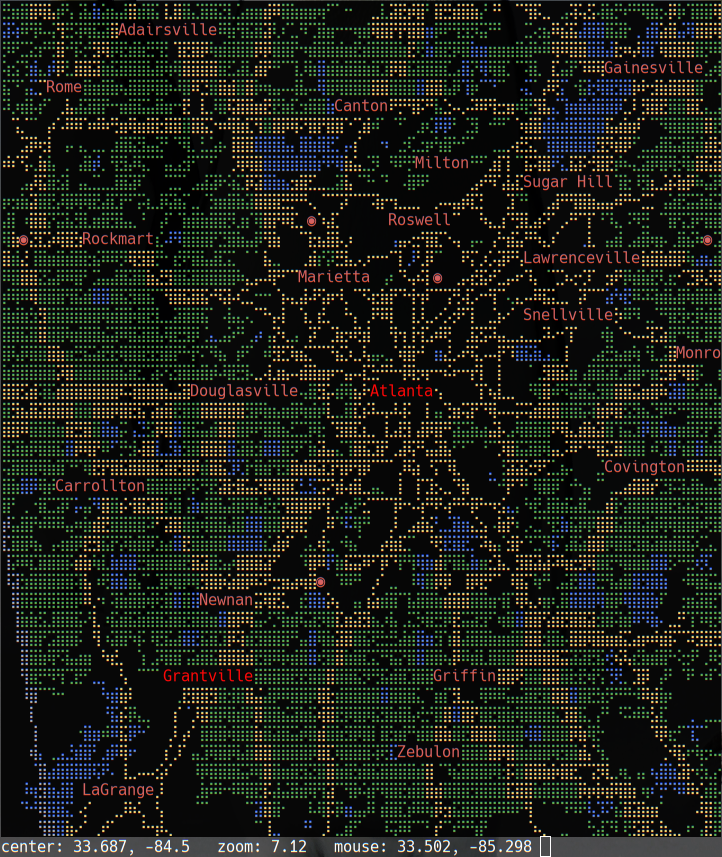
\includegraphics[width=.4\linewidth]{media/tui-mapscii.png}
    \hfill
    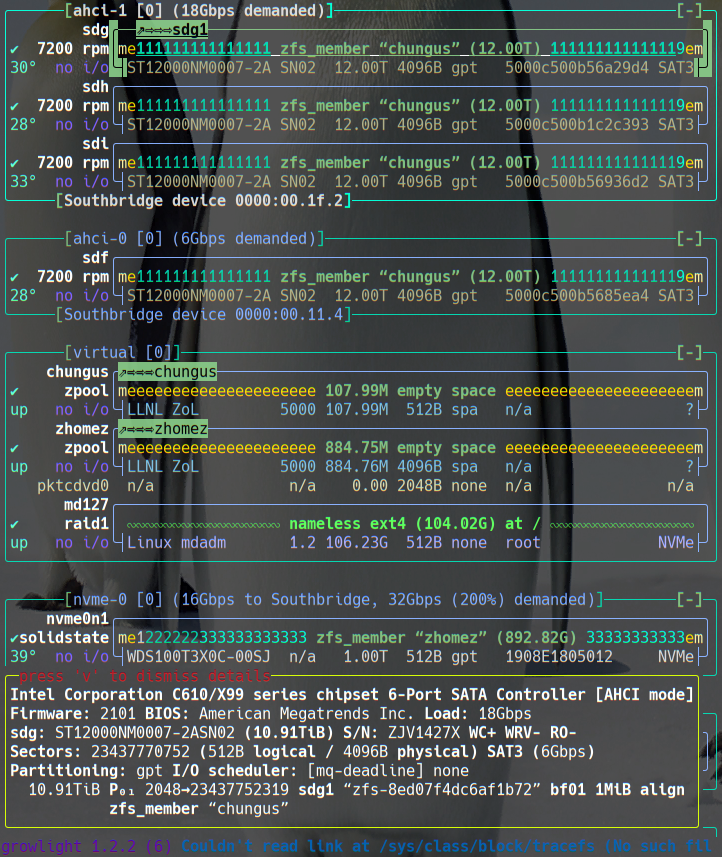
\includegraphics[width=.4\linewidth]{media/tui-growlight.png}
    \caption[Non-NCURSES TUIs: Mapscii and Growlight.]{\texttt{mapscii}, a
    node.js application, blew my mind when I first saw it. The high resolution
    is achieved by using Braille characters, trading away some color control.
    \texttt{growlight} began life as an NCURSES C program, but was ported to
    Notcurses in 2019.}
  \label{fig:notncurses-tuis}
\end{figure}

Implementing a TUI will usually require, at a minimum:
\begin{denseitemize}
\item{Receiving input from user devices, including keyboards and mice,}
\item{some manner of user configuration widgets (menus, etc.),}
\item{watching for some other event(s) from the system, and},
\item{juggling these various components without wastefully polling, nor
       introducing undue latency, and enforcing safe synchronized access to
       the graphics interface.}
\end{denseitemize}

Perhaps most terrifyingly, it will require user interface design. Notcurses
attempts to assist with this by providing numerous ready-made widgets.

This text has two goals:
\begin{denseitemize}
\item{To provide a firm footing for design and implementation of character
    graphics and TUIs, elucidating the dimensions of design, and difficulties
    to avoid, and}
\item{to serve as ``narrative reference'' for my Notcurses library, and as
    a starting place for newcomers.}
\end{denseitemize}

\begin{figure}[!htbp]
\centering 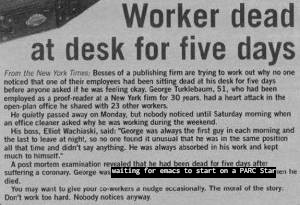
\includegraphics[width=.5\linewidth]{media/emacs-xerox.jpg}
  \caption{Put not your trust in hackers making a fetish of Xerox PARC.}
  \label{fig:xeroxemacs}
\end{figure}

Cell graphics are primarily the realm of \textit{terminals}, which for the
purposes of this book encompass any means by which input devices act to provide
input to a some process generating glyph-based output to a display. This
includes hardware terminals (inputs integrated with displays, connected to a
computer as a unit), operating system consoles (text-mode interfaces operating
with the graphics engine directly connected to the terminal driver), terminal
multiplexers (tools like \texttt{screen}, \texttt{tmux}, and \texttt{mosh},
providing a memory-persistent virtual terminal with which other terminals can
interact), and terminal emulators (applications which present a virtual
terminal atop the shard input and raster output methods of a graphical user
environment). There's some vagueness and variety involved with these terms.

At its heart, a terminal is a line discipline plus two buffers: an input buffer
to collect user-generated events (possibly from multiple devices), and an
output buffer to be processed and displayed. The buffers can be modeled as byte
streams, mutating the output at the time of their display (in contrast to e.g.\
a framebuffer, where the entirety of the screen is present at any given time).
The earliest terminals were electromechanical teletypes, reproducing their
input as line-based print on paper. These gave rise to ``dumb terminals''
(cathode-ray displays with a scrolling rectilinear output area). ``Smart
terminals'' followed, with the ability to move freely within their display
area, and also to extract and act upon ``control codes'' embedded in the output
stream. The text modes of the first video cards were designed around the
capabilities of these smart terminals. This brings us to the present, wherein
high-powered LED displays have their pixels summoned up and ordered into
formations suitable for the reconstruction of 1970s technology (a history of
terminals is presented in Appendix~\ref{sec:terminals}).

The machine on which I'm typing this contains a
TU104 GPU consisting of over thirteen billion 12nm-process transistors,
rendering its output to a 3440x1440 (almost five megapixel) display. Deep
within its silicon heart remains a VGA 80x25 text mode engine, inherited
largely unchanged from the EGA, the CGA, the IBM Monochrome Display Adapter,
and before that smart terminals\footnote{As early as 1971, the block-oriented
IBM 3277 Model 2 ``green screen'' shipped with 80x24.}.


I generally use this modern marvel to drive terminal emulators of 80 columns.

\newpage
%%%%%%%%%%%%%%%%%%%%%%%%%%%%%%%%%%%%%%%%%%%%%%%%%%%%%%%%%%%%%%%%%%%%%%%%

\section{Using direct mode with standard I\/O}

Many tools don't intend to be full-screen TUI applications, but instead
implement that purest of UNIX interfaces: newline-delimited text, oblivious
to screen geometry, capable of being fed as input to other, similar programs.
For such tools, the full Notcurses capabilities are neither necessary nor
desirable. These programs are typically non-interactive: humans might peruse
their outputs and prepare their inputs, but they effectively run as a batch
task.

 Such tools might still want to colorize and otherwise style their output, at
least when being output to a terminal. This can be accomplished using the
\texttt{ncdirect} subset of Notcurses, and is known as \textit{direct mode}. Direct
mode functionality should not usually be mixed with other Notcurses calls.
Unlike full Notcurses, there is no explicit rendering step in direct mode, and
it is intended to be mixed among other use of standard I/O. Essentially, direct
mode ``styles your \texttt{printf()}s.'' Similarly to full Notcurses, direct mode
requires a valid and correct terminfo database entry, supplied via either the
\texttt{termtype} parameter to \texttt{notcurses\_directmode()} or the \texttt{TERM} environment
variable. It does \textit{not}, however, require any particular encoding nor
even a call to \texttt{setlocale()} (full Notcurses requires a properly-configured
ASCII or UTF-8 locale).

Enter direct mode via a call to \texttt{notcurses\_directmode()} with a successful
return of a non-\texttt{NULL} pointer to \texttt{struct ncdirect}:

\begin{listing}[!htbp]
\begin{minted}{C}
// Initialize a direct-mode notcurses context on the connected terminal at 'fp'.
// 'fp' must be a tty. You'll usually want stdout. Direct mode supportes a
// limited subset of notcurses routines which directly affect 'fp', and neither
// supports nor requires notcurses_render(). This can be used to add color and
// styling to text in the standard output paradigm. Returns NULL on error,
// including any failure initializing terminfo.
struct ncdirect* notcurses_directmode(const char* termtype, FILE* fp);
\end{minted}
\end{listing}

It is typical to invoke this function as \texttt{notcurses\_directmode(NULL, stdout)}.
In this case, the terminal type must be present in the \texttt{TERM} environment
variable (this should have been done by the terminal). The buffering and
blocking status of \texttt{fp} will not be changed. \texttt{NULL} is returned for any number
of possible errors. Otherwise, the \texttt{struct ncdirect} is ready to go, and should
be cleaned up with \texttt{ncdirect\_stop()}:

\begin{listing}[!htbp]
\begin{minted}{C}
// Release 'nc' and any associated resources. 0 on success, non-0 on failure.
int ncdirect_stop(struct ncdirect* nc);
\end{minted}
\end{listing}

Between these two calls, inject stylizing control codes into the \texttt{FILE*} with
the following API (the \texttt{stylebits} values are detailed in Chapter~\ref{sec:attribute}):

\begin{listing}[!htbp]
\begin{minted}{C}
int ncdirect_bg_rgb8(struct ncdirect* n, unsigned r, unsigned g, unsigned b);
int ncdirect_fg_rgb8(struct ncdirect* n, unsigned r, unsigned g, unsigned b);
int ncdirect_fg(struct ncdirect* n, unsigned rgb);
int ncdirect_bg(struct ncdirect* n, unsigned rgb);
int ncdirect_styles_set(struct ncdirect* n, unsigned stylebits);
int ncdirect_styles_on(struct ncdirect* n, unsigned stylebits);
int ncdirect_styles_off(struct ncdirect* n, unsigned stylebits);
int ncdirect_clear(struct ncdirect* n);
\end{minted}
\end{listing}

As detailed in Chapter~\ref{sec:channels}, the terminal has a ``default foreground color''
and ``default background color''. Use these functions to return to them.

\begin{listing}[!htbp]
\begin{minted}{C}
int ncdirect_fg_default(struct ncdirect* n);
int ncdirect_bg_default(struct ncdirect* n);
\end{minted}
\end{listing}

Direct mode allows the cursor to be moved in two-dimensional space, and
provides helpers for determining the terminal geometry. Either \texttt{y} or
\texttt{x} may be specified as -1 to maintain location on the associated axis.

\begin{listing}[!htbp]
\begin{minted}{C}
int ncdirect_dim_x(const struct ncdirect* nc);
int ncdirect_dim_y(const struct ncdirect* nc);
int ncdirect_cursor_move_yx(struct ncdirect* n, int y, int x);
\end{minted}
\end{listing}

\subsection{Example: presenting \textit{\textcolor{blue}{House} of Leaves}}

Mark Z. Danielewski's experimental 2000 novel \textit{\textcolor{blue}{House} of Leaves}\cite{danielewski2000house} prints each
instance of the word \textcolor{blue}{house} in blue, even when it is a subword:

\begin{figure}[!htbp]
\centering 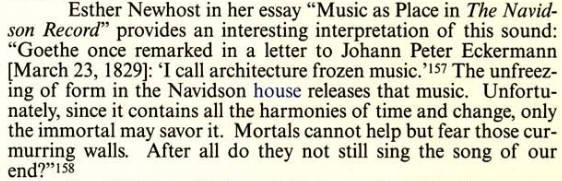
\includegraphics[width=.5\linewidth]{house-blue.png}
\caption{An excerpt from page 123 of \textit{\textcolor{blue}{House} of Leaves}.}
\label{fig:houseofleaves}
\end{figure}

We can easily write code to reproduce this effect for standard input and output.
The following works as expected (see Figure~\ref{fig:houseout}):

\begin{listing}[!htbp]
\inputminted[]{C}{code/hol-formatter.c}
\caption{\texttt{hol-formatter.c}}
\end{listing}

There are a few things worth noting about the code above. First, observe how
much of the logic is devoted to checking and propagating errors! Perhaps
contrary to common expectation, reliable code--especially when that code's
primary effect is to write to stdout--generally needs to check the results of
e.g. \texttt{printf()} (what happens if we're redirected to a file, and
the disk is full?). A language making use of exceptions would reduce if not
eliminate this nonsense.

\begin{figure}[!htbp]
\centering 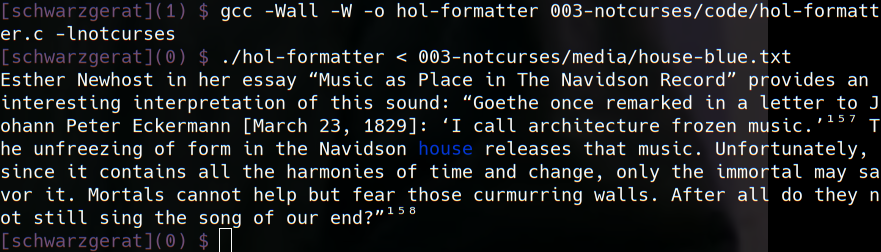
\includegraphics[width=.75\linewidth]{hol-formatted.png}
\caption[\texttt{hol-formatter} as run on OCRd input.]{\texttt{hol-formatter} as run on our input. We use \texttt{tesseract} for OCR, with solid results.}
\label{fig:houseout}
\end{figure}

We don't switch from blue to some random color, because we don't know the
background color of the terminal. Hard to believe as it is, some people don't
favor a dark terminal background. If the terminal background was white, and we
had just used e.g. \texttt{ncdirect\_fg(n, 0xffffff)}, text following
``\textcolor{blue}{house}'' would be invisible.

One might observe that a user with a blue background will have invisible
``\textcolor{blue}{house}'' text. This is true, and there's no great solution
to it. It is not generally possible to discover the RGB values of the default
colors. I suppose all one can do is rest easy, serene in the belief that people
with chromatic backgrounds deserve whatever happens to them.

\subsection{Example: colorizing a dumb game}

Imagine we've written the simple guessing game in Listing~\ref{list:guessgame}.

\begin{listing}[!htbp]
\inputminted[]{C}{code/hilostdio.c}
\caption{\texttt{hilostdio.c}}
\label{list:guessgame}
\end{listing}

The correct approach for a player is binary search, and for an $N$-bit
\texttt{long}, we expect to guess the number in no more than $N$ tries. Let's
color the output to indicate how bad of a guess was offered. We'll use red for
low guesses, blue for high guesses, and break the 256 shades of each (assuming
the other two components to be fixed) uniformly across the $N$ levels of
logarithmic distance\footnote{This would be a good place to employ \gls{gamma correction}.}.
If we wanted to do this (see Listing~\ref{list:hilodirect}) without direct use of RGB color,
we'd either need accept fewer shades, or be forced to reprogram the palette.

\begin{listing}[!htbp]
\inputminted[]{C}{code/hilodirect.c}
\caption{\texttt{hilodirect.c}}
\label{list:hilodirect}
\end{listing}

Stepping through the orders of magnitude\footnote{\texttt{\_\_builtin\_clzl()}
is a compiler intrinsic for \textit{count leading zeroes}. Exhaustive methods
for fast clzl can be found in \cite{hackerdelight}. Demonstrating that
absolute value of the difference of leading zeroes is a $lg_{2}$ difference
is left as an exercise for the reader.}, we get the expected gradient
(Figure~\ref{fig:colorguess}). Were we to actually play, the response would
converge to a balanced, strong green as we approached the correct answer.

\begin{figure}[!htbp]
\centering 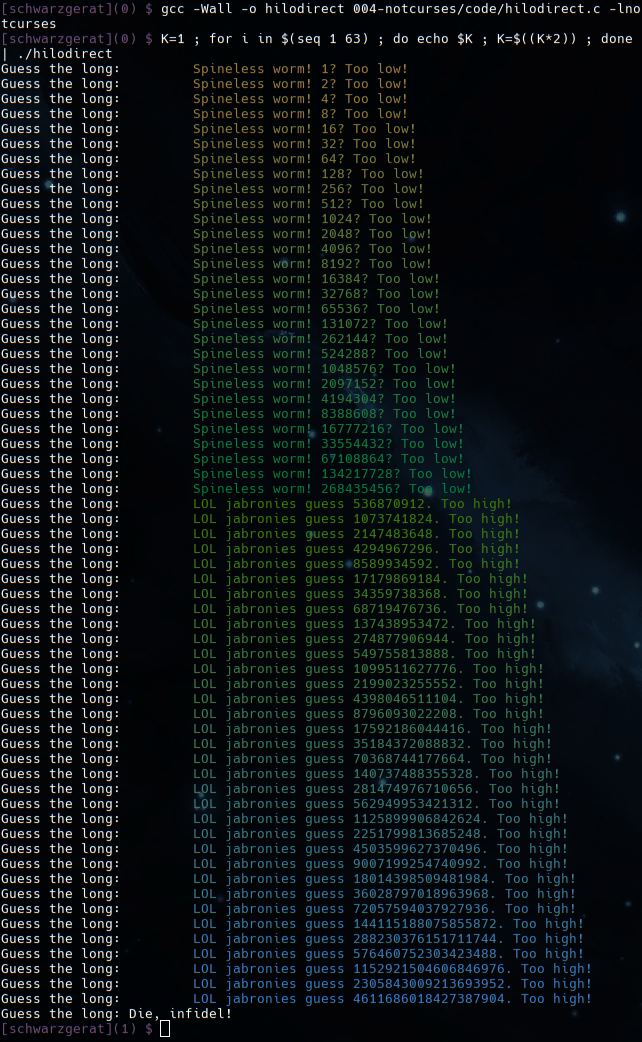
\includegraphics[width=.75\linewidth]{media/hilodirect.png}
\caption{Colorized output from~\texttt{hilodirect.c}.}
\label{fig:colorguess}
\end{figure}

\subsection{Advanced coëxistence with stdio}
It is most common to initialize Notcurses with \texttt{stdout}, whether in
direct mode or fullscreen mode. This isn't the only way to operate, though.
By opening the tty directly using \texttt{/dev/tty}\cite{tty4}, and providing
this \texttt{FILE*} to Notcurses, a program passing its standard output to
another process can make concurrent use of Notcurses on the display, in either
direct or fullscreen mode. This is how the \texttt{notcurses-pipe} program
works\footnote{See \url{https://github.com/dankamongmen/notcurses/issues/381}.}.

For programs that need to write to the terminal, but want to ``overlay'' some
Notcurses, fullscreen mode won't work (though the program could be run in an
\texttt{ncprocess} widget; see Chapter~\ref{sec:uiwidgets}). Direct mode, however, is
a possibility. I've not yet written the example\footnote{Send me patches! Or
I'll do it\ldots eventually \url{https://github.com/dankamongmen/notcurses/issues/382}.}, but it is possible to, for
instance, periodically acquire the current cursor position, move elsewhere on
the screen, update a HUD, and return to the departure position. Scrolling could
be addressed by retaining a copy of any obliterated output. This would suffer
a startup period of one screen, during which the area scrolled above the HUD
would be cleared. This could be avoided by aligning the HUD with the top of
the terminal.

\newpage

%%%%%%%%%%%%%%%%%%%%%%%%%%%%%%%%%%%%%%%%%%%%%%%%%%%%%%%%%%%%%%%%%%%%%%%%
\section{Using fullscreen mode}
From this chapter forward, we will be using the fullscreen mode of Notcurses,
opening up all of its capabilities. This comes at a cost: while fullscreen mode
is being used, it is not safe to use standard I/O in conjunction with the
terminal controlled by Notcurses. Doing so is likely to (at a minimum) corrupt
the screen. If \texttt{stdout} and \texttt{stderr} are attached to the same
terminal (as they usually are in an interactive session), and \texttt{stdout}
is provided to Notcurses, output to \texttt{stderr} will corrupt the display
just as thoroughly as output to \texttt{stdout}. If your fullscreen Notcurses
program intends to log to \texttt{stderr}, you should first ensure that that
it has been redirected or is otherwise going somewhere different than
\texttt{stdout}. Note that simply rerendering the output will \textit{not}
necessarily clean up corruption, even following \texttt{ncplane\_erase()}
operations, since Notcurses optimizes its rendering based on its concept of the
screen. A call to \texttt{notcurses\_refresh()} will be necessary to sync the
the physical screen to Notcurses's concept thereof.

It is possible for the screen to be corrupted by external agents. For this
reason, Ctrl+L is by tradition bound to screen redrawing. You should hook this
input up to \texttt{notcurses\_refresh()} unless you have good reasons not to
do so (this is not default behavior of Notcurses only because Notcurses does
not itself read input). It is sadly not possible for such corruption to be
efficiently and generally detected.

It is possible for the attached terminal to be resized, especially (but not
only) for terminal emulators in GUI windowing environments\footnote{This could
also happen when refitting a \texttt{screen} or \texttt{tmux} session.
Even on the Linux or FreeBSD console, this can happen due to a change in video
resolution.}. Notcurses can detect such events, and synthesizes
\texttt{NCKEY\_RESIZE} inputs in response to them. If the screen shrinks, the
excess data relative to the constant origin will no longer be displayed (i.e.
the material in the upper left will be retained). If the screen is enlarged,
any data uncovered will be displayed, and the new area will otherwise be empty.
Some widgets can intelligently resize themselves in the face of screen
geometry changes (see Chapter~\ref{sec:uiwidgets}).

Notcurses prepares a given terminal for fullscreen mode in \texttt{notcurses\_init()}

\begin{listing}[!htbp]
\begin{minted}{C}
// Initialize a notcurses context on the connected terminal at 'fp'. 'fp' must
// be a tty. You'll usually want stdout. Returns NULL on error, including any
// failure initializing terminfo.
struct notcurses* notcurses_init(const notcurses_options* opts, FILE* fp);

// Destroy a notcurses instance, restoring the terminal to its original state.
int notcurses_stop(struct notcurses* nc);
\end{minted}
\end{listing}

Before calling \texttt{notcurses\_init()} (and usually as one of the first lines
of the program) it is necessary to set the current locale via the standard
library function \texttt{setlocale()}. A coverage of ANSI/ISO C locales is beyond
the scope of this text, but it is usually sufficient to call
\texttt{setlocale(LC\_ALL, "")}, relying on the user's configured \texttt{LANG}
environment variable. Notcurses only supports those locales using
US-ASCII or UTF-8 encodings (see Chapter~\ref{section:unicode} for more
information on character encodings), and its capabilities on US-ASCII
are \textit{severely} constrained. \texttt{notcurses\_init()} will return an
error for any other encoding (see Figure~\ref{fig:encodingfail}).

\begin{figure}[!htbp]
\centering 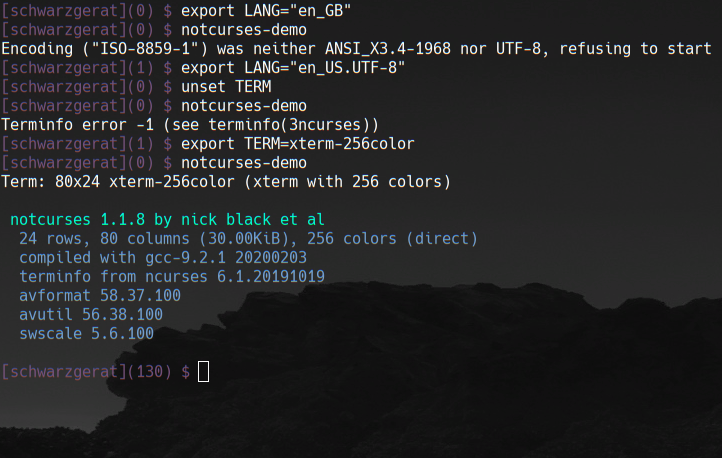
\includegraphics[width=.7\linewidth]{media/notcurses-init-fails.png}
\caption{Notcurses refusing to start due to an unsupported character encoding.}
\label{fig:encodingfail}
\end{figure}

By default (assuming the \texttt{enter\_ca\_mode} terminfo capability is expressed),
Notcurses attempts to enter the ``\gls{smcup}''. Using the alternate screen
implies:
\begin{denseitemize}
\item{The screen will be cleared upon entry,}
\item{Output will not be appended to the scrollback buffer, and}
\item{On exit, output will be cleared.}
\end{denseitemize}
Whether or not the original screen contents are restored is terminal-dependent
(if the \texttt{non\_rev\_rmcup} terminfo capability is defined, the original
contents will \textit{not} be restored). This can be useful, but some users
don't like it, so it's wise to expose this via a configuration option.
Disabling use of the alternate screen can be done via the
\texttt{notcurses\_options} field \texttt{inhibit\_alternate\_screen}.

Successful creation of a \texttt{struct notcurses} implies the existence of
a \texttt{struct ncplane}, the ``standard plane''\footnote{\texttt{ncplane}s,
discussed in depth in Chapter~\ref{ncplane}, are the fundamental drawing surfaces of Notcurses.}.
This standard plane cannot be destroyed without destroying the containing
Notcurses context, nor can it be moved or resized by the user. Its size always
matches Notcurses's conception of the terminal's screen size, and its origin
always corresponds precisely to the terminal's origin. Aside from these
restrictions, the standard plane is a drawable surface like any other
\texttt{ncplane}---it can be moved along the z-axis, written to with arbitrary
glyphs and styles, made transparent, etc.

Once you're done using a \texttt{struct notcurses}, it's important to destroy
it with \texttt{notcurses\_stop()}, even if your process exits abnormally. By
default, Notcurses registers signal handlers for most fatal signals. These
handlers will call \texttt{notcurses\_stop()} and then pass the signal to the
orginal actions. You can disable this with the \texttt{no\_quit\_sighandlers}
field of \texttt{notcurses\_options}, but there aren't very many good reasons
to do so.

\subsection{The \texttt{notcurses\_options} structure}
The first parameter to \texttt{notcurses\_init()} is a (possibly \texttt{NULL})
\texttt{notcurses\_options}. This structure has been defined such that the
default options are equivalent to a zero-initialized structure. Passing \texttt{NULL}
is thus equivalent to passing a zero-initialized \texttt{notcurses\_options}.
The fields therein include:
\begin{denseitemize}
\item{\texttt{const char* termtype}: The name of the terminfo database entry to
    use. If \texttt{NULL}, the value of the environment variable \texttt{TERM}
    is used. Failure to initialize the terminfo database will result in a
    \texttt{notcurses\_init()} failure.} A defined but invalid or suboptimal
    entry will result in garbage, missing output, poor performance, reduced
    colors, and unsightly weight gain.
\item{\texttt{bool inhibit\_alternate\_screen}: As noted above, this prevents
    Notcurses from making use of the alternate screen, even if the \texttt{enter\_ca\_mode}
    terminfo capability is defined. It's best to wire this up to a user-managed
    option. Not using the alternate screen can look weird upon return to the
    shell (see Figure~\ref{fig:altscreen}).

\begin{figure}[!htbp]
\centering 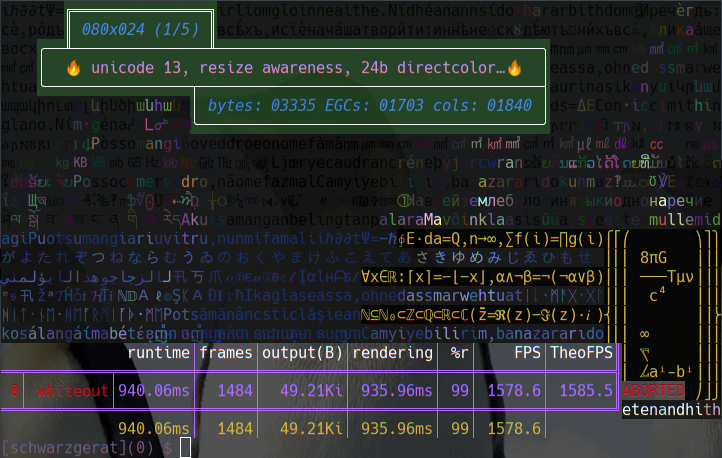
\includegraphics[width=.7\linewidth]{media/no-alternate-screen.png}
\caption[Inhibiting use of the alternate screen.]{\texttt{notcurses-demo} can be invoked with \texttt{-k} to avoid
  using the alternate screen. Here, we see its output left on the screen as
  we return to our shell.}
\label{fig:altscreen}
\end{figure}
  }
\item{\texttt{bool retain\_cursor}: Notcurses hides the cursor by default.
    Set this to keep the cursor visible (the cursor can be turned on and off
    at runtime with \texttt{notcurses\_cursor\_enable()} and
    \texttt{notcurses\_cursor\_disable()}).}
\item{\texttt{bool suppress\_banner}: At startup, Notcurses emits some
    diagnostics and/or warnings, including version information and details
    about the current terminal. At shutdown, it prints performance statistics.
    These outputs \textit{do not} go to the alternate screen. Set this
    field to disable these outputs, but be aware that doing so might hide
    important warnings (see Figure~\ref{fig:banner}).

    \begin{figure}[!htbp]
      \centering 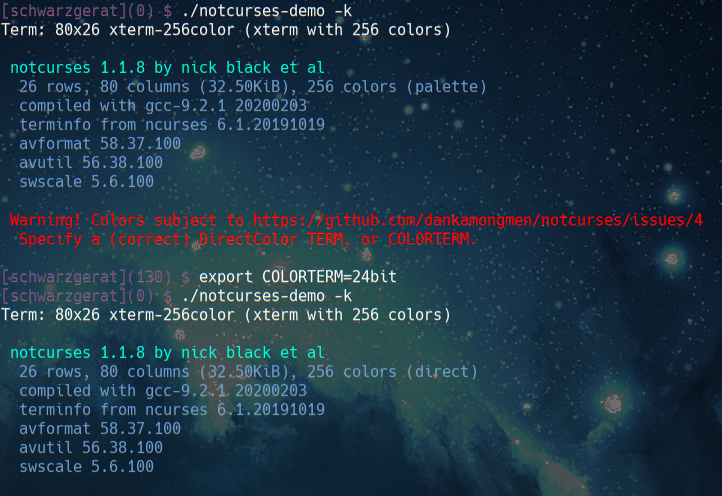
\includegraphics[width=.7\linewidth]{media/notcurses-banner.png}
      \caption[Notcurses initialization warnings.]{Initializing Notcurses without 24-bit color support will
        generate a warning, hopefully provoking your users to set it up.}
      \label{fig:banner}
    \end{figure}
}
\item{\texttt{bool no\_quit\_sighandlers}, \texttt{bool no\_winch\_sighandler}:
    As noted above, Notcurses by default registers signal actions for the normally fatal
    \texttt{SIGABRT}, \texttt{SIGINT}, \texttt{SIGQUIT}, and \texttt{SIGSEGV}.
    These handlers will call \texttt{notcurses\_stop()} before propagating the
    signal to the original actions. This is usually desirable, as the screen
    will not otherwise be restored to its previous state. In addition, \texttt{SIGWINCH}
    is caught in order to generate \texttt{NCKEY\_RESIZE} inputs. If you
    disable these handlers, you'll almost certainly want to replace them with
    similar functionality.}
\item{\texttt{FILE* renderfp}: If not \texttt{NULL}, this designates a file
    handle open for writing. In addition to the terminal, each rendered scene
    will be written to this file. This is intended for debugging.}
\end{denseitemize}

\subsection{Functions on \texttt{notcurses} objects}

Output is not written to this top-level \texttt{struct notcurses}---that's
done with \texttt{ncplane}s---but there are a number of functions
available for these objects. Acquiring an \texttt{ncplane} for output can be
done by grabbing a reference to the standard plane, or creating a new plane.
New planes are always inserted into the top of the z-axis. All user-created
planes can be destroyed in one call with \texttt{notcurses\_drop\_planes()} (note
that it is not necessary to call this prior to \texttt{notcurses\_stop()}; the
latter cleans up all resources associated with the context).

\begin{listing}[!htbp]
\begin{minted}{C}
// Get a reference to the standard plane (one matching our current idea of the
// terminal size) for this terminal. The standard plane always exists, and its
// origin is always at the uppermost, leftmost cell of the terminal.
struct ncplane* notcurses_stdplane(struct notcurses* nc);

// Create a new ncplane at the specified offset (relative to the standard plane)
// and the specified size. The number of rows and columns must both be positive.
// This plane is initially at the top of the z-buffer, as if ncplane_move_top()
// had been called on it. The void* 'opaque' can be retrieved (and reset) later.
struct ncplane* ncplane_new(struct notcurses* nc, int rows, int cols,
                            int yoff, int xoff, void* opaque);

// Return the topmost ncplane, of which there is always at least one.
struct ncplane* notcurses_top(struct notcurses* n);

// Destroy any ncplanes other than the stdplane.
void notcurses_drop_planes(struct notcurses* nc);
\end{minted}
\end{listing}

Reading input is a per-context operation, performed with \texttt{notcurses}
objects. It is discussed in detail in Chapter~\ref{sec:input}. When reading
input, we might get the synthesized event \texttt{NCKEY\_RESIZE}\footnote{This
event is generated upon receipt of a \texttt{SIGWINCH} signal, SIGnifying WINdow
CHange.}. This indicates that the terminal has been resized, and we ought call
\texttt{notcurses\_resize()}\footnote{Really? \textbf{FIXME} \url{https://github.com/dankamongmen/notcurses/issues/367}.}.
As discussed earlier, sometimes the display is externally corrupted. It's thus
a good idea to hook some UI event (usually Ctrl+L) to \texttt{notcurses\_refresh()},
which redraws every cell on the display according to the internal Notcurses
framebuffer.

\begin{listing}[!htbp]
\begin{minted}{C}
// Refresh our idea of the terminal's dimensions, reshaping the standard plane
// if necessary. Without a call to this function following a terminal resize
// (as signaled via SIGWINCH), notcurses_render() might not function properly.
// References to ncplanes (and the egcpools underlying cells) remain valid
// following a resize operation, but the cursor might have changed position.
int notcurses_resize(struct notcurses* n, int* restrict y, int* restrict x);

// Refresh the physical screen to match what was last rendered (i.e., without
// reflecting any changes since the last call to notcurses_render()). This is
// primarily useful if the screen is externally corrupted.
int notcurses_refresh(struct notcurses* n);
\end{minted}
\end{listing}

\begin{listing}[!htbp]
\begin{minted}{C}
// Get a human-readable string describing the running notcurses version.
const char* notcurses_version(void);
\end{minted}
\end{listing}

Finally, \texttt{notcurses\_render()} synthesizes a terminal's worth of current
state out of all your virtual objects, schedules an optimized list of escape
sequences and encoded characters, and blits the result to the terminal. Only
through \texttt{notcurses\_render()} (and transitively through its callers) ought
your program write to the actual terminal, and only \texttt{notcurses\_render()}
has any bearing on what the user sees. Between calls, you are free to do whatever
you want in terms of moving, reordering, creating, writing upon, and destroying
planes. There will be no flicker or tearing; what you last rendered remains on
the screen. When you've got your stack how you want it, and only then, invoke
\texttt{notcurses\_render()}. It is an exclusive function---any concurrent use
of the same \texttt{struct notcurses} is undefined.

\begin{listing}[!htbp]
\begin{minted}{C}
// Make the physical screen match the virtual screen. Changes made to the
// virtual screen (i.e. most other calls) will not be visible until after a
// successful call to notcurses_render().
int notcurses_render(struct notcurses* nc);
\end{minted}
\end{listing}

\subsection{Reading, rendering, rasterizing, and writing}
\label{sec:rendering}

Understanding how Notcurses translates its data structures into a terminal
display is critical for reasoning about your program in general, and particularly
relevant for maximizing performance.

During initialization of a terminal, unless \texttt{suppress\_banner} is supplied
in the \texttt{notcurses\_options}, \texttt{notcurses\_init()} will print some
diagnostics to stdout, and flush the output buffer. Notcurses maintains an
internal virtual framebuffer, containing the state of the terminal as believed
to exist\footnote{Do not confuse this with the standard plane. This framebuffer
reflects rendering and rasterizing, not the output API.}. It is initialized in
\texttt{notcurses\_init()} to an empty matrix of cells, each cell having the
default foreground and background.

What happens next depends on whether the ``alternate screen'' (as described
earlier) is employed. If so, the terminal will be immediately cleared.
Otherwise, the terminal will not be altered until the first call to
\texttt{notcurses\_render()}. That first call, however, will write to every
cell of the terminal, effectively clearing any existing output. The upshot is
that it is not possible to integrate preexisting data into your TUI, regardless
of whether the alternate screen is used. This reflects the impossibility of
portably discovering the state of the terminal.

Subsequent to the first call, Notcurses---having written them---has a concept
of the display's contents. From that point on, screen updates will write only
to changed (``damaged'') cells. When only parts of the screen have changed,
this saves a tremendous amount of work. On an 80x45 terminal, if only a 10x10
region of cells have changed, we reduce our bandwidth by about
95\%\footnote{10x10 is only 2.7\% of 80x45, but there is overhead due to moving
the cursor to the region, and then positioning the cursor at the end of each
line of the region.}. These savings are multiplicative:

\begin{denseitemize}
\item{Notcurses doesn't have to \texttt{write()} the data (memory copy).}
\item{The terminal doesn't have to \texttt{read()} the data (memory copy).}
\item{The terminal doesn't need to process the data (assorted work).}
\item{The terminal doesn't need to write to the display (memory copy).}
\end{denseitemize}

Whether a cell has been updated is decided at rasterization time. Writing to
that cell between calls to \texttt{notcurses\_render()} does not necessarily
mean the cell will be considered damaged when it comes time to write. If the
cell has been damaged, it will be emitted, and the virtual framebuffer internal
to Notcurses will be updated.

Solving for the desired state of the screen is \textit{rendering}, and this is
the first step of \texttt{notcurses\_render()}. Solving for the screen means
solving for the current state of every cell, given our ordered set of
\texttt{ncplane}s. Solving for a cell means determining the extended grapheme
cluster to be rendered, determining the attributes to be applied to that EGC,
and determining the colors in which it ought be displayed. The higher a plane
is on the z-axis, the more it can impact these solutions:

\begin{denseitemize}
\item{The EGC and attribute are determined by the first plane intersecting with
      the cell having a non-null EGC at the intersecting coordinate. If there is
    no such intersecting EGC, the EGC is null, and the attribute is
    \texttt{NCSTYLE\_NORMAL}.} Null EGCs are rendered as spaces (i.\ e.\ entirely
    background color).
\item{The foreground color is determined by the first instance of a
    \texttt{CELL\_ALPHA\_OPAQUE} foreground color, or an instance of the
    default foreground color, or an instance of a palette-indexed foreground
    color, as well as any \texttt{CELL\_ALPHA\_HIGHCONTRAST} or \texttt{CELL\_ALPHA\_BLEND}
    foreground colors encountered along the way. If there is no such intersecting
    terminator, the foreground color is the color as calculated thus far. It is
    not possible to exhaust all intersecting planes without encountering some
    influence on the foreground color, since the standard plane intersects with
    all display cells. If \texttt{CELL\_ALPHA\_HIGHCONTRAST} is in play, the
    calculated color is then blended to stand out against the calculated background
    color.}
\item{The background color is determined in the same way as the foreground color,
    except without the complicating possibility of \texttt{CELL\_ALPHA\_HIGHCONTRAST}.}
\end{denseitemize}

Once a cell is solved, Notcurses needn't continue inspecting lower planes at
that coordinate. Once all cells are solved, rendering is complete, and any
planes left over can be skipped entirely. Until then, Notcurses steps down from
one plane to the next, starting at the topmost plane, and updates its solution
for any intersecting unsolved cells. It is thus generally more performant to
``hide'' planes at the bottom of the stack, ideally behind a large opaque plane,
rather than moving them beyond the boundaries of the visible window. Likewise,
planes ought be no larger than necessary, so that they intersect with the
minimum number of cells.

Having rendered the scene, \textit{rasterization} serializes a buffer to write
to the terminal, minimizing the amount of data by moving the cursor over undamaged
regions. This is the second step of \texttt{notcurses\_render()}. Writing this
data to the terminal as it's generated is a bad idea for several reasons: it can
provoke unnecessary context switches, it results in partially-updated displays,
and it definitely involves more system calls. Notcurses instead collects it in
one or more large allocations.

Proceeding cell-by-cell from the upper left to the lower right, Notcurses
compares the rendering solution set to its internal framebuffer. If a given row
is entirely undamaged, it can be skipped. Upon discovering the leftmost damage
on a row, an absolute cursor update is performed to the damaged cell. At each
damaged cell, the EGC will be emitted, along with any necessary styling
information. It is only necessary to emit styling escapes when they change, i.\ e.\ we
can emit multiple EGCs having the same style after only issuing the appropriate
escapes once. An RGB change takes about 14 bytes, a palette index change
takes about 6, and reverting to the default 2. For single-byte simple (ASCII)
EGCs, an RGB foreground and background represent 2800\% overhead per cell!
Eliding styling escapes is thus an important secondary optimization (it's of
course most desirable to not update the cell at all).

The upshot is that holding styling constant across a horizontal stretch is
very desirable if that range's content is going to be changing. The most
pathological input to Notcurses is text that changes its foreground and background
on a cell-to-cell basis, especially when specified as RGB, that change from
render to render. Certain terminal emulators in particular respond to the
resulting deluge of RGB escapes very poorly (see Appendix~\ref{sec:termshade}).
As examples, see the \texttt{highcontrast} and \texttt{grid} demos of
\texttt{notcurses-demo}---a large \texttt{xterm} can be brought to its knees
by these routines.

Each subsequent range of undamaged cells on a line can be skipped over with
cursor movements, but as the skip length approaches 1, it becomes less and
less advantageous to do so. Rendering performance can be very roughly
categorized as inversely proportional to the product of:

\begin{denseitemize}
\item{color changes across the rendered screen,}
\item{planar depth before an opaque glyph and background are locked in,}
\item{number of UTF-8 bytes composing the rendered glyphs, and}
\item{screen geometry.}
\end{denseitemize}

With these buffers in hand, \texttt{notcurses\_render()} completes its task by
writing them to the terminal. This almost certainly means copying
them into a kernel buffer from which the terminal will then (following at
least one context switch and two system calls) read. Writing does not,
then, necessarily mean that the display has actually been updated, or even
that the terminal has read the data. If the terminal doesn't empty the buffer
quickly enough, however, you'll eventually run out of room and block. It is
thus critical to understand that \textbf{\texttt{notcurses\_render()} can block
for arbitrary amounts of time}\footnote{But see
\url{https://github.com/dankamongmen/notcurses/issues/214}.}. Furthermore,
if the terminal reads two renderings' worth of output at the same time, it is
likely to immediately enter the final state---you must not assume that a successful
\texttt{notcurses\_render()} is necessarily displayed within any arbitrary time,
or indeed that it corresponds with any displayed frame.

With those unhappy truths said, modern workstations ought have no problem pushing
notcurses onto commodity hardware at maximum framerates, with the terminal
faithfully reproducing each rendered scene. Even small microcontrollers ought
be able to render notcurses without user-perceptible latency. On a powerful
desktop with non-pathological output, it's easy to render in excess of
ten thousand frames per second, far beyond the refresh capabilities of any
existing monitor.

\subsection{Statistics}

notcurses tracks statistics across its operation, and a snapshot can be
acquired using the \texttt{notcurses\_stats()} function. This function cannot
fail.

\begin{listing}
\begin{minted}{C}
typedef struct ncstats {
  // purely increasing stats
  uint64_t renders;          // number of successful notcurses_render() runs
  uint64_t failed_renders;   // number of aborted renders, should be 0
  uint64_t render_bytes;     // bytes emitted to ttyfp
  int64_t render_max_bytes;  // max bytes emitted for a frame
  int64_t render_min_bytes;  // min bytes emitted for a frame
  uint64_t render_ns;        // nanoseconds spent in notcurses_render()
  int64_t render_max_ns;     // max ns spent in notcurses_render()
  int64_t render_min_ns;     // min ns spent in successful notcurses_render()
  uint64_t cellelisions;     // cells we elided entirely thanks to damage maps
  uint64_t cellemissions;    // cells we emitted due to inferred damage
  uint64_t fgelisions;       // RGB fg elision count
  uint64_t fgemissions;      // RGB fg emissions
  uint64_t bgelisions;       // RGB bg elision count
  uint64_t bgemissions;      // RGB bg emissions
  uint64_t defaultelisions;  // default color was emitted
  uint64_t defaultemissions; // default color was elided

  // current state -- these can decrease
  uint64_t fbbytes;          // total bytes devoted to all active framebuffers
  unsigned planes;           // number of planes currently in existence
} ncstats;

// Acquire an atomic snapshot of the notcurses object's stats.
void notcurses_stats(struct notcurses* nc, ncstats* stats);

// Reset all cumulative stats (immediate ones, such as fbbytes, are not reset).
void notcurses_reset_stats(struct notcurses* nc, ncstats* stats);
\end{minted}
\caption{Notcurses exports a comprehensive set of statistics.}
\end{listing}

Timings for renderings are across the breadth of \texttt{notcurses\_render()}:
they include all per-render preprocessing, output generation, and dumping of
the output (including any sleeping while waiting on the terminal).

The notcurses drawing algorithm logically starts by zeroing out a
\textit{solutions array} of booleans. When this array is all true, we've solved
for each cell of the output, and can stop. It then walks down the z-axis. For
each plane encountered, any unsolved cells with which that plane interacts are
adjusted, and the solution array updated if appropriate. Note that there will
always be at least one plane interacting with each visible coordinate, due
to the default plane. The process of filling a solutions matrix is referred to
as rendering.

The next step is \textit{rasterization}. Rather than moving down the z-axis, we now
move to the right and down on the screen, starting from the upper left corner.
At each cell, we examine the solutions matrix and the previous contents of the
cell. If they are the same, no output is emitted. If they are different, the
new glyph is written to the output, following any necessary cursor movements
and styling codes. notcurses attempts to minimize the total amount of data
written by eliding unnecessary color and style specifications, and moving the
cursor over large unchanged areas.

Using the ``default color'' as only one of the foreground or background requires
emitting the \texttt{op} escape followed by the appropriate escape for changing the
fore- or background (since \texttt{op} changes both at once).

Certain EGCs are understood to be all-foreground or all-background.
\texttt{U+2588 FULL BLOCK} is all foreground. \texttt{U+0020 SPACE} is all
background. When such a character is used, notcurses will emit whichever
character can take advantage of the current color.

\newpage

%%%%%%%%%%%%%%%%%%%%%%%%%%%%%%%%%%%%%%%%%%%%%%%%%%%%%%%%%%%%%%%%%%%%%%%%
\section{A simple notcurses render\slash event loop}
I'm not typically a fan of example-based instruction, preferring to build things
up from formal axioms. Following chapters will effect such an approach. First,
however, let's work a semi-substantial example covering a varied set of
Notcurses routines. We're going to create seven planes, one for each kind
of tetrimino, and map an image file to the background. We'll add support for
switching between the pieces, rotating them, and sliding them around the
screen. Finally, we'll deal with collisions, and fluid handling of
screen resizings. In the course of doing so, you'll learn several important
Notcurses techniques:

\begin{denseitemize}
\item{Drawing and rotating these tetriminos will involve colors, gradients, and
      transparencies. The former are fundamental drawing tools. The latter is
      all one needs for sprites.}
\item{Mapping the background will involve image decoding, scaling, and blitting.}
\item{We'll cover most of what's worth knowing regarding input.}
\end{denseitemize}

This example will be picked up and further developed in the Tetris case study
of Chapter~\ref{section:casestudy}\footnote{Were you aware that there is a
standard for Tetris clones? There is indeed\cite{tetris}.}.

\begin{figure}[!htbp]
\centering 
\includegraphics[width=.5\linewidth]{media/tetriminos.png}
\caption{Piping hot tetriminos, fresh from~\textit{Spiritus Mundi}.}
\label{fig:tetriminos}
\end{figure}

Almost every Notcurses program will take the same general form, an \textit{event+render loop}:

\begin{denseitemize}
\item{Essential screen elements are laid down.}
\item{Initial state is discovered and added to the display.}
\textbf{begin loop} 
\item{Some thread, perhaps the only thread in the process, watches
    for user input. Other threads might be collecting system events that will
    change the state. Either way, an event occurs.}
\item{Thread(s) receiving events perform any necessary mutual exclusion.}
\item{Thread(s) manipulate the Notcurses virtual state via \texttt{ncplane} manipulations.}
\item{\texttt{notcurses\_render()} is called by a single thread.}
\textbf{end loop}
\item{The process terminates.}
\end{denseitemize}

\subsection{Example: moving tetriminos with a keyboard}

We could load the pieces as images from files, but given the simplicity of the
sprites, it feels simpler to just hardcode them in our source. I don't want to
leave my text editor\footnote{Vim. See Figure~\ref{fig:xeroxemacs}.} to muck
with images when we can do everything in fewer than ten lines, even in a naïve
and wasteful encoding (Listing~\ref{list:tetrimino-data}).

\begin{listing}[!htbp]
\inputminted[]{C}{code/tetrimino-data.h}
\caption{The seven canonical tetriminos (from~\texttt{tetrimino.c}).}
\label{list:tetrimino-data}
\end{listing}

To warm up and get limber, let's create seven \texttt{ncplane}s, one for each type
of tetrimino. We'll lay them out in a 2-3-2 formation. This layout will be
sloppy, for now: our function
\texttt{tetrimio\_plane()} accepts a piece ID and a coordinate.
The plane it creates has its origin at this coordinate.
We're not yet adjusting for the size of the planes themselves when coming
up with these coordinates---this shifts everything down and to the right from
symmetric divisions of the screen, as you'll see.

\begin{figure}[!htbp]
\centering 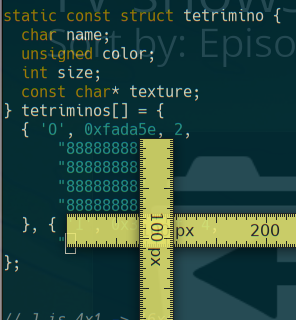
\includegraphics[width=.5\linewidth]{media/screenruler.png}
\caption{Font aspect ratios center around 0.5.}
\label{fig:aspectratio}
\end{figure}

We use two display rows per game row but four display columns per game column.
This reflects what is, at least on my display and font, pretty much a 0.5
aspect ratio (Figure~\ref{fig:aspectratio}).

\begin{listing}[!htbp]
\inputminted[]{C}{code/tetrimino-display.h}
\caption{Creating a single tetrimino (from~\texttt{tetrimino.c}).}
\label{list:tetrimino-display}
\end{listing}

There are a few essential things to
take away from Listing~\ref{list:tetrimino-display}:

\begin{denseitemize}
\item{Each time we call \texttt{ncplane\_putsimple()}, the cursor is advanced
      the expected amount. If we were calling \texttt{ncplane\_putegc()} with
      a multicolumn grapheme cluster, the cursor would be advanced multiple
      columns.}
\item{Between rows, we need move the cursor ourselves, since we're skipping over
      part of the plane (this isn't true for several of the pieces, but the
      cursor update is a trivial operation, not worth avoiding).}
\item{The cursor is always initialized to the origin of a new plane, and coordinates
      supplied to \texttt{ncplane\_} functions are relative to the plane,
      \textit{not} the terminal. Coordinates can be translated among planes
      using \texttt{ncplane\_translate()}.}
\item{We only have ASCII characters in the textures right now. Were we to
      introduce any multibyte UTF-8---and we may well do so, for e.\ g.\ the
      Box Drawing Characters---the \texttt{strlen()} we size our rows by here
      would no longer fly. We'd need use \texttt{mbstowcs()}, or redefine the
      textures as \texttt{wchar\_t} arrays and use \texttt{wcslen()},
      or change up our encoding\footnote{We go with the third option, as you'll see.}. \textfrench{\textit{Rien n'est simple, mais tout est facile\ldots}}}
\end{denseitemize}

\begin{listing}[!htbp]
\inputminted[]{C}{code/tetrimino-draw.h}
\caption{Distributing the tetriminos with ``flying-v'' technique (from~\texttt{tetrimino.c}).}
\label{list:tetrimino-draw}
\end{listing}

\begin{listing}[!htbp]
\inputminted[]{C}{code/tetrimino-main.h}
\caption{A one-shot, display-only \texttt{main()} (from~\texttt{tetrimino.c}).}
\label{list:tetrimino-main}
\end{listing}

Our \texttt{main()} sets the locale, initializes the terminal, and draws the
seven pieces (Listings~\ref{list:tetrimino-draw} and~\ref{list:tetrimino-main}).
Each piece has a one-letter name; for now, we draw with those glyphs. The
pieces are monochromatic. This renders familiar shapes in the correct colors
(Figure~\ref{fig:tetriminos-1}), but other than that, it's (like most classic
Curses programs) kinda fugly. I wouldn't want to play with these pieces.

\begin{figure}[!htbp]
  \centering
  \begin{minipage}{0.30\textwidth}
    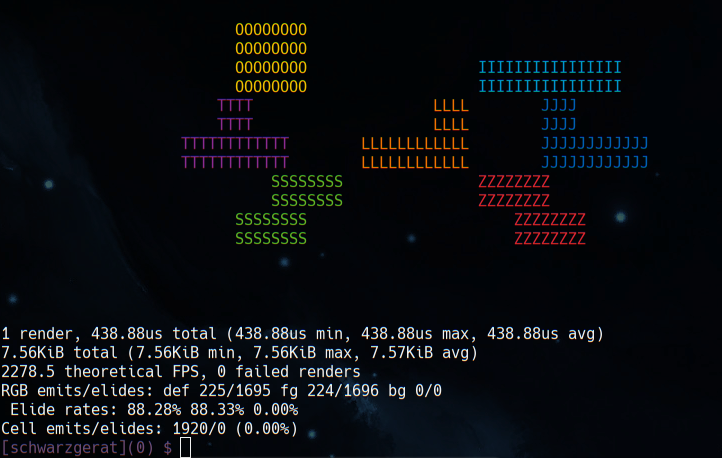
\includegraphics[width=1\linewidth]{media/tetriminos-1.png}
    \caption{Unspeakably foul.}
    \label{fig:tetriminos-1}
  \end{minipage}\hfill
  \begin{minipage}{0.30\textwidth}
    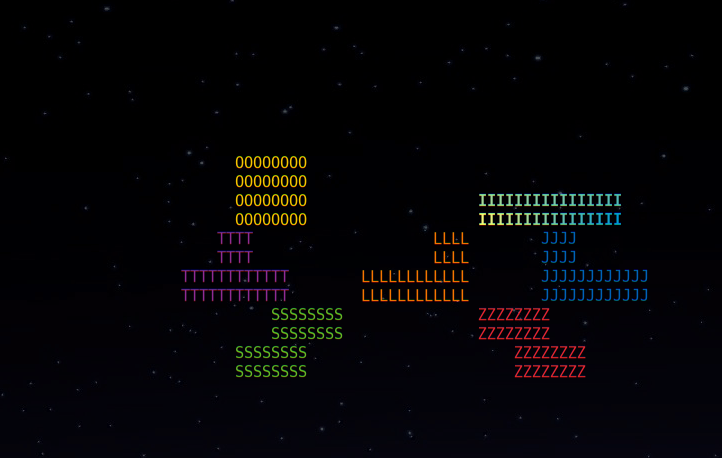
\includegraphics[width=1\linewidth]{media/tetrimino-gradient1.png}
    \caption{Adding a gradient.}
  \end{minipage}\hfill
  \begin{minipage}{0.30\textwidth}
    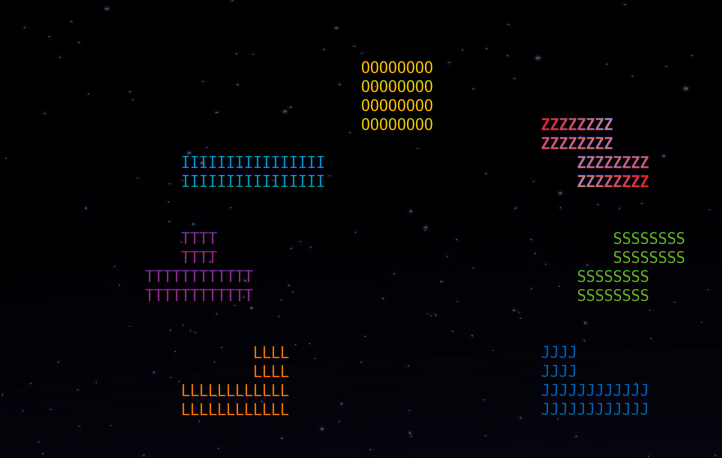
\includegraphics[width=1\linewidth]{media/tetrimino-gradient2.png}
    \caption{Linear expansion.}
  \end{minipage}\hfill
\end{figure}

This is hardly a render/event loop; in fact it's not a loop at all. If we were
using the alternate screen, we wouldn't see our output before flashing back to
the normal screen. Let's go ahead and hook up input. We'll be controlling one
of the tetriminos at a time---the selected piece will use boldface, and have its
color brightened\footnote{Note how we use two distinct indicators. On a monochromatic
display, we need the bold, and on a display which can't do bold, maybe we get a
color difference. Also, we want bold even if we have color, because until we
see the base color, there's no reason to think of the initial selection as
``bright''.}. We do so (Listing~\ref{list:tetrimino-switch}) with a pair of
helpers---\texttt{reduce()} and \texttt{highlight()}--- which drive the common
\texttt{blast()}. \texttt{blast()} makes use of two new functions,
\texttt{ncplane\_format()} and \texttt{ncplane\_stain()}. They allow the
attributes and channels, respectively, of a rectangular region to be changed
without altering other components. The corresponding glyph-only output routines
are likewise described in (Chapter~\ref{sec:staining}).

\begin{listing}[!htbp]
\inputminted[]{C}{code/tetrimino-switch.h}
\caption{Switching between pieces (from~\texttt{tetrimino-input.c}).}
\label{list:tetrimino-switch}
\end{listing}

While we're making things prettier, let's replace
those letters with some classy box-drawing characters, and improve on this
layout. We can do some simple algebraic extensions and get some linear spacing,
but it's just as easy to use trigonometric functions and get an approximation
to a circle. This is especially valuable as the terminal geometry changes; our
fixed linear scalings would break down as the display aspect changes, but a
good ol' circle will work on any sufficient radius
(Listing~\ref{list:tetrimino-drawcircle}).

\begin{listing}[!htbp]
\inputminted[]{C}{code/tetrimino-drawcircle.h}
\caption{Trigonometric layout: simpler, yet more accurate (from~\texttt{tetrimino-input.c}).}
\label{list:tetrimino-drawcircle}
\end{listing}

Since there's nothing else going on, it's trivial to process \texttt{stdin} in
a blocking fashion from our main thread. Let's add the code to track a selected
piece, visually highlight it, and process input (Listing~\ref{list:tetrimino-inputcore}).
The space bar will advance among the pieces in one direction,
and Tab in the other. The arrow keys and vi keys will translate the selected
piece in four directions. The parentheses will rotate the piece $\frac{\pi}{2}$ radians
clockwise and counterclockwise.

\begin{listing}[!htbp]
\inputminted[]{C}{code/tetrimino-inputcore.h}
\caption{Core input dispatch (from~\texttt{tetrimino-input.c}).}
\label{list:tetrimino-inputcore}
\end{listing}

Of course, when there's no other activity, things are easy. Quite often, we'll
have some periodic concurrent activity. Let's say we wanted to make the non-selected
tetriminos slowly rotate. The rotation isn't difficult; Notcurses provides
that functionality for you. But you don't want the rotation synced to input
activity, and you're hardly the kind of know-nothing what-not that would
busy loop on a nonblocking input interface, right? I hope you don't consider
yourself ``green'' if that's the case, because you're burning dinosaurs out
of sheer laziness. Let's do it right. There are of course four canonical
solutions to the problem of interleaving a set of asynchronous file descriptor-based
inputs against a set of periodic requirements; let's refresh ourselves:

\begin{denseitemize}
\item{No holds barred, take no prisoners state machine. No quarter asked.
    None given. Certainly the most \textit{enjoyable} choice of the four, the
    one closest to the nature of the machine, and the option with the most
    built-in job security. Casting off the crutch of the process scheduler, we
    execute in a single thread, carefully programming our
    \texttt{epoll()}\cite{epoll7} or \texttt{kqueue()}\cite{kqueue2} timeouts
    against a hierarchal, hashed timer wheel\cite{timerwheels}. As Alan Cox
    said, ``Computers are state machines. Threads are for people who don't
    understand state machines.''\footnote{Or did he? I can't find the original
    to cite. I wonder what the hell happened to Alan Cox.} Limited to a single
  CPU\ldots\ which probably isn't a problem here, but isn't exactly a great foundation
  on which to build our cathedral, \textfrench{\textit{n'est-ce pas?}}.}
\item{Two threads enter, one thread \texttt{exit()}s (hehehehe). We block on
    async I/O in our main thread. Another thread runs a timer wheel---for this,
    a loop around a \texttt{clock\_nanosleep()} will suffice. They
    lock against one another to avoid corrupting the screen or otherwise
    embarassing ourselves. The solution reeks of Java, but will work well
    enough, and any programmer---maybe even a Java programmer---ought be able
    to walk in and pick it up.}
\item{POSIX signaled timers. Noooooooooooooooooooooooooooooooooooooo.}
\item{Timer I/O multiplexing. Probably the best solution for a program of true
    scope, and in no way unfit for the task at hand. On Linux, you'll want
    \texttt{timerfd\_create()} and friends. On FreeBSD, look for \texttt{EVFILT\_TIMER}.
    Throw that into the appopriate I/O multiplexor call, spin it out among a
    few threads if you feel so inclined\cite{libtorque}, and call it a day.
  The only real disadvantage here is a lack of portability.}
\end{denseitemize}

Some will ask, ``Sounds dank, but what about on this shiny operating system I
purchased from Applooglesoft? Look, I can speak to it! Sirana, diminish my
freedoms and spy on me!'' I could give two shits about your closed-source
operating system. I presume you can purchase cloud-based Timers as a Service
(TaaS) or something.

We can now cycle through the pieces, and move the piece we've selected around
on the screen. Grab one and move it towards another piece. Experimentation will
reveal that each piece has a~\gls{boundingbox}, that there is a total ordering
among the seven pieces, and that a piece below another piece's bounding box is
robbed of its color (Figure~\ref{fig:tetrimino-badplane}). Recall from
Chapter~\ref{sec:rendering} how we solve for each coordinate of the display
grid: the EGC is a dimension distinct from the coloring channels. Each of the
planes we create is rectilinear, with the piece drawn using Unicode
\texttt{U+2588 FULL BLOCK}, and the other cells left unwritten. The foreground
for our pieces is an RGB color, and for the other cells is the default terminal
color. Upon intersecting with a lower plane, the lower plane's EGC is chosen for
rendering, but the foreground color is default terminal color (white in my
example). So the piece underneath flipping to white while another piece is
nearby makes perfect sense. The solution is simple: we set the foreground
transparent for the base character of each plane. Foreground calculation will
now bypass the plane where we haven't drawn, and the distorted plane regains
its expected colors (Figure~\ref{fig:tetrimino-trans}). Takeaway: by default, planes
obstruct only color, not glyphs.

\begin{figure}[!htbp]
  \centering
  \begin{minipage}{0.30\textwidth}
    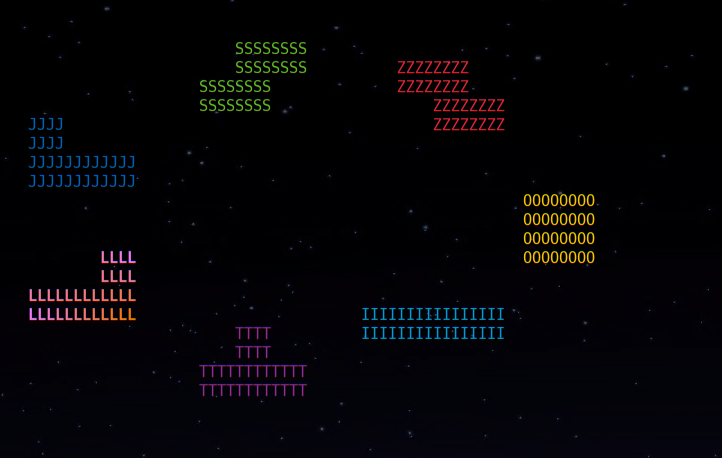
\includegraphics[width=1\linewidth]{media/tetrimino-gradient3.png}
    \caption{Trigonometry!}
  \end{minipage}\hfill
  \begin{minipage}{0.30\textwidth}
    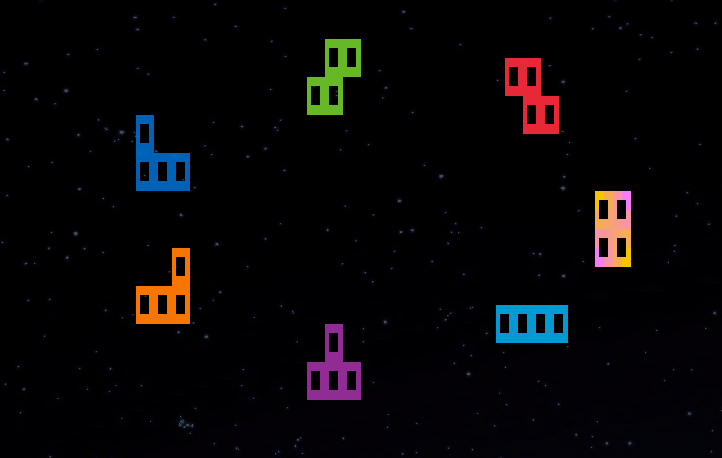
\includegraphics[width=1\linewidth]{media/tetrimino-gradient4.png}
    \caption{Unicode Blocks.}
  \end{minipage}\hfill
  \begin{minipage}{0.30\textwidth}
    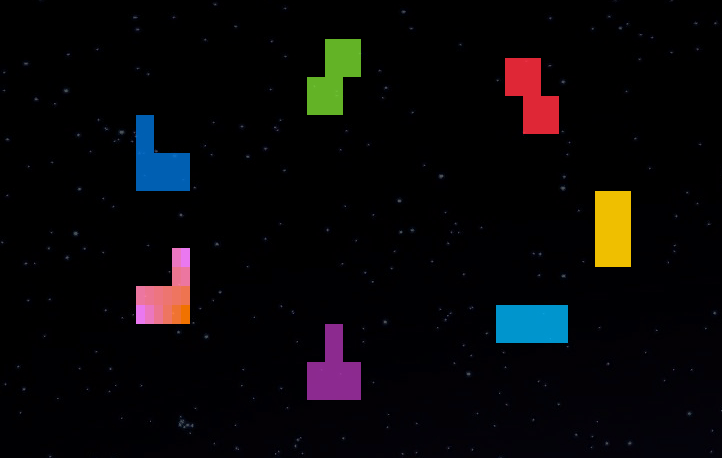
\includegraphics[width=1\linewidth]{media/tetrimino-gradient5.png}
    \caption{Better blocks.}
  \end{minipage}\hfill
\end{figure}

\begin{figure}[!htbp]
  \begin{minipage}{0.30\textwidth}
    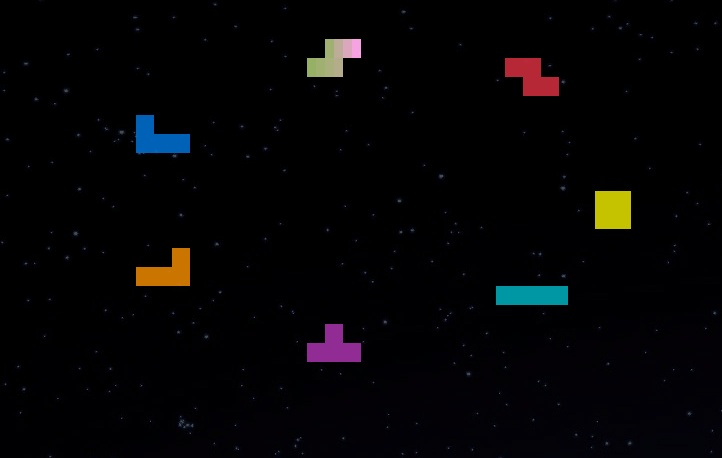
\includegraphics[width=1\linewidth]{media/tetrimino-gradient6.png}
    \caption{Adjusting for cell aspect ratio.}
  \end{minipage}\hfill
  \begin{minipage}{0.30\textwidth}
    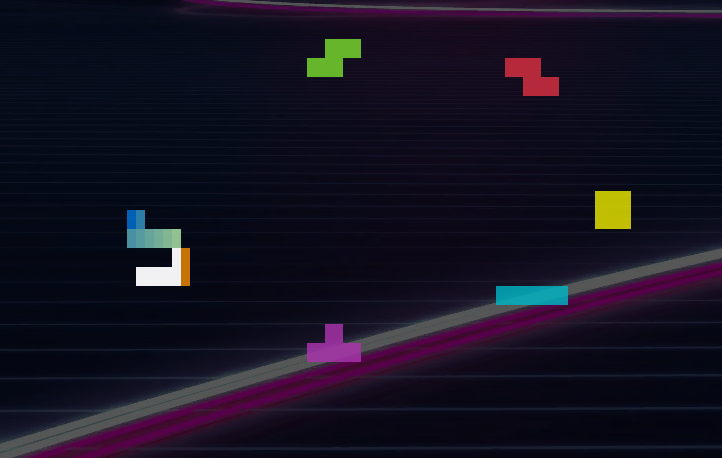
\includegraphics[width=1\linewidth]{media/tetrimino-gradient7.png}
    \caption{Undesirable plane interaction.}
    \label{fig:tetrimino-badplane}
  \end{minipage}\hfill
  \begin{minipage}{0.30\textwidth}
    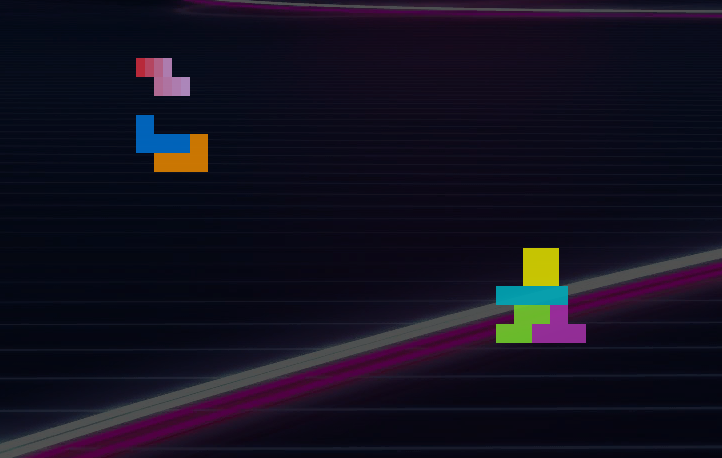
\includegraphics[width=1\linewidth]{media/tetrimino-gradient8.png}
    \caption{Resolve it with transparent planes.}
    \label{fig:tetrimino-trans}
  \end{minipage}\hfill
\end{figure}

\begin{listing}[!htbp]
\inputminted[]{C}{code/tetrimino-databox.h}
\begin{minted}{C}

\end{minted}
\inputminted[]{C}{code/tetrimino-displayutf8.h}
\caption{Improving appearance with Unicode Block Elements (from~\texttt{tetrimino-input.c}).}
\label{list:tetrimino-displayutf8}
\end{listing}

Adding a background image is simple. We'll render it to the standard plane, our
``background'' for now (remember, newly created planes are placed at the top of
the z axis). Despite decoding the image \textit{after} creation of the pieces,
the pieces are thus not hidden. There is no need to inform Notcurses of the
image's format, nor parameters thereof. Simply provide the file name and target
rendering plane, and we're off. See Chapter~\ref{sec:libav} for a full treatment
of multimedia in Notcurses.

\begin{listing}[!htbp]
\inputminted[]{C}{code/tetrimino-background.h}
\caption{Throwing in a background (from~\texttt{tetrimino-input.c}).}
\label{list:tetrimino-background}
\end{listing}

To rotate the unselected pieces, we'll go ahead and spawn a POSIX thread. We'll
thus need lock against piece selection. We've been leaving all the end-of-process
cleanup in the capable hands of~\texttt{notcurses\_stop()}, but it can't go
terminating threads for us, and it in any case wouldn't be safe to do so while
said thread was calling into Notcurses! First, add a marshaling struct to share
some state (Listing~\ref{list:tetrimino-tetmarsh}). We'll use POSIX
cancellation\footnote{Which isn't anywhere near as bad as it's sometimes made out to be.
Find the places where you don't want to be cancelled. Each such place needs a
cleanup handler pushed/popped around it, or cancellation disabled for its
breadth. Things get a little counterintuitive with
cancellable-but-uninterruptible system calls, but that's nothing if you came up
on BSD signals. It's hardly the most offensive wart on the great hairy ass
that is ANSI/ISO C, and---heresy, I know---I honestly prefer (most of) the
POSIX model to (most of)
the threading introduced in \CC11.} to blast the rotator thread, and~\texttt{pthread\_join()}
it to ensure safe passage through shutdown.

\begin{listing}[!htbp]
\inputminted[]{C}{code/tetrimino-tetmarsh.h}
\caption{Marshaling structure for shared state (from~\texttt{tetrimino-input.c}).}
\label{list:tetrimino-tetmarsh}
\end{listing}

\begin{listing}[!htbp]
\inputminted[]{C}{code/tetrimino-thread.h}
\caption{Spin them doggies (from~\texttt{tetrimino-input.c}).}
\label{list:tetrimino-thread}
\end{listing}

As a final touch, let's slide a dark, translucent plane underneath the
selected piece, making it more visible. We create this plane prior to the
pieces, ensuring it's below all of them (but above the background). We set it
black, and its alpha to \texttt{CELL\_ALPHA\_BLEND}. This way it won't entirely
block out the background underneath the selected piece, but it will dim it,
its black blending into the grey tones underneath. The piece is unaffected.

\begin{listing}[!htbp]
\inputminted[]{C}{code/tetrimino-box.h}
\caption{Set the selection off with a coaster (from~\texttt{tetrimino-input.c}).}
\label{list:tetrimino-box}
\end{listing}

\begin{figure}[!htbp]
  \centering
  \begin{minipage}{0.30\textwidth}
    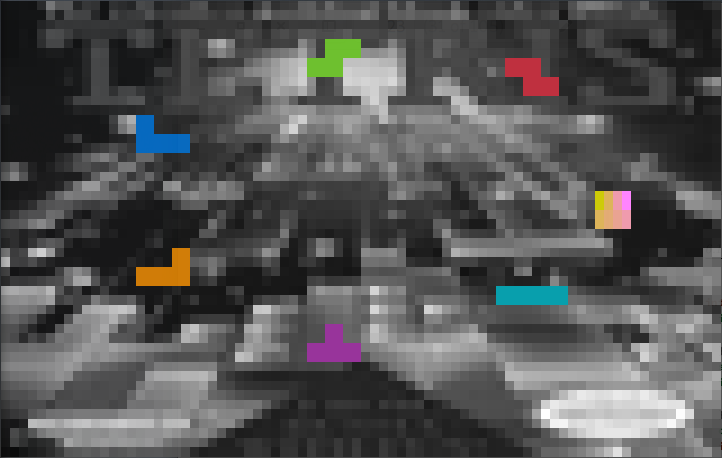
\includegraphics[width=1\linewidth]{media/tetrimino-bg.png}
    \caption{Background image, greyscaled.}
    \label{fig:tetrimino-bg}
  \end{minipage}\hfill
  \begin{minipage}{0.30\textwidth}
    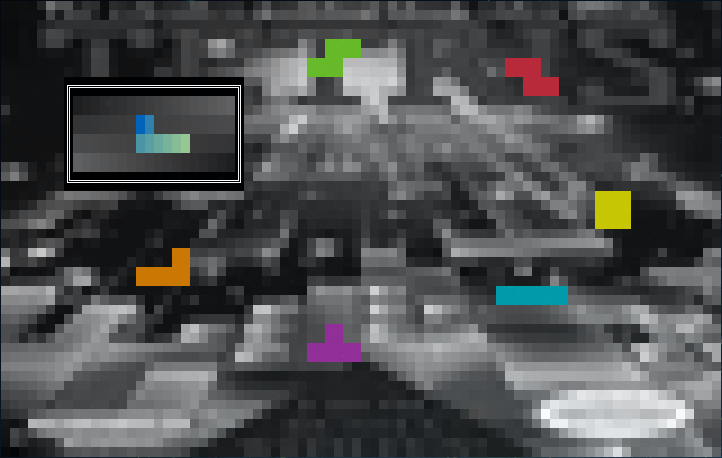
\includegraphics[width=1\linewidth]{media/tetrimino-bgbox.png}
    \caption{Opaque highlight box.}
  \end{minipage}\hfill
  \begin{minipage}{0.30\textwidth}
    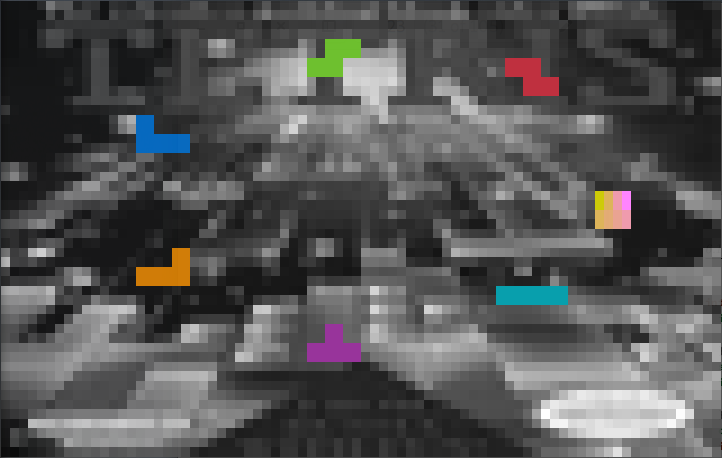
\includegraphics[width=1\linewidth]{media/tetrimino-bg.png}
    \caption{Rotation thread enabled\textbf{FIXME}.}
  \end{minipage}\hfill
\end{figure}

\begin{listing}[!htbp]
\inputminted[]{C}{code/tetrimino-inputmain.h}
\caption{Putting it all together (from~\texttt{tetrimino-input.c}).}
\label{list:tetrimino-inputmain}
\end{listing}

\pagebreak
\newpage
%%%%%%%%%%%%%%%%%%%%%%%%%%%%%%%%%%%%%%%%%%%%%%%%%%%%%%%%%%%%%%%%%%%%%%%%

\section{The mechanics of a tty}
\label{section:tty}
\textbf{FIXME FIXME acquisition of a tty (getty->login, ssh->pty),
  internals of kernel tty/pty devices, session groups, signal distribution,
  \texttt{/dev/tty} and \texttt{/dev/ttyXX}s}
\textbf{FIXME FIXME other stuff}
\subsection{Escape codes ANSI and otherwise}
\label{sec:escapes}
My diagrams are adapted in part from those of Linus Akesson\cite{ttydemystified}.
\textbf{FIXME diagrams!}

In a relic from teletypes, ISO 646, ISO 2022, and ECMA-35 described use of
non-destructive backspace to produce composed characters from spacing ones.
This had been eliminated by ISO 4873, ECMA-43, and ISO 8859.

\textbf{FIXME FIXME other stuff}

\newpage
%%%%%%%%%%%%%%%%%%%%%%%%%%%%%%%%%%%%%%%%%%%%%%%%%%%%%%%%%%%%%%%%%%%%%%%%

\section{Character encodings and glyphs}
\label{section:unicode}
We'll be well-served by becoming familiar with our core building
blocks---character sets and their rasterized forms. Even if we were to shrink
the character cell to a single pixel, we'd still need write one or another
character into it, and emit a control code to stylize it\footnote{I've seen
this idea bandied about as if it's a serious suggestion. Besides the fact
that it won't work in a console, escapes are \textit{far} less efficient than
canvases or OpenGL display lists; if your plan involves using ANSI escape
sequences to drive a 1920x1080 display via roughly two million 1x1 character
cells, you're not going to space today, or maybe ever\cite{upgoerfive}.}.
\subsection{The Universal Character Set}
\begin{center}
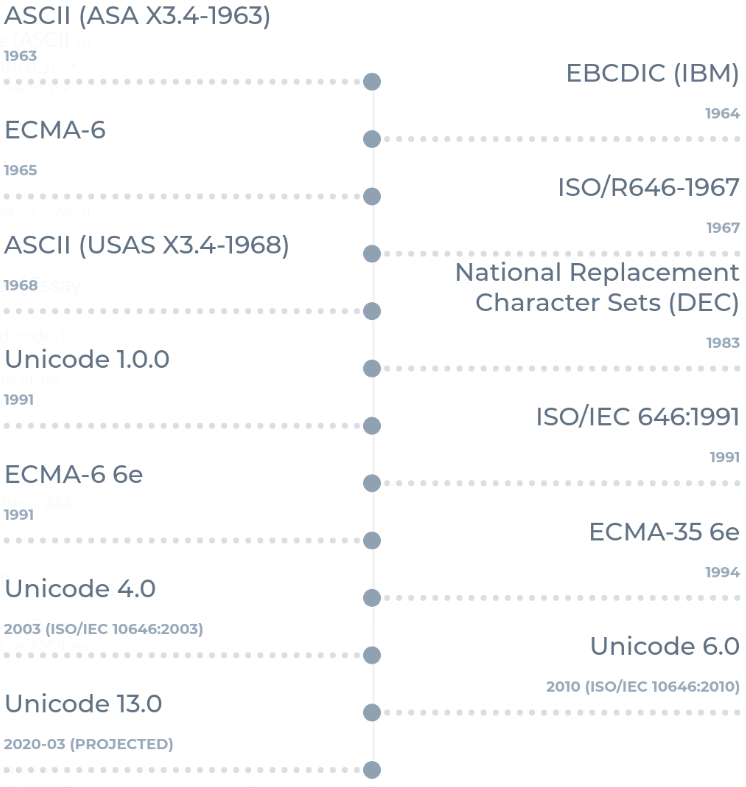
\includegraphics[width=.9\linewidth]{media/charset-timeline.png}
\end{center}

\footnote{Once upon a time, these other sixteen planes were known as the
  Astral Planes\cite{astralplanes}.}
\subsection{UTF-8}
\subsection{Stupid Unicode tricks}
\textbf{FIXME} cyclic groups, reversals, zalgo, \url{http://qaz.wtf/u/}

\subsection{Fixed-width fonts ain't so fixed}

Notcurses assumes that all glyphs occupy widths which are an integral multiple
of the smallest possible glyph's cell width (aka a ``fixed-width font'').
Unicode introduces characters which generally occupy two such cells, known as
wide characters (though in the end, width of a glyph is a property of the
font). It is not possible to print half of such a glyph, nor is it generally
possible to print a wide glyph on the last column of a terminal.

Notcurses does not consider it an error to place a wide character on the last
column of a line. It will obliterate any content which was in that cell, but
will not itself be rendered. The default content will not be reproduced in such
a cell, either. When any character is placed atop a wide character's left or
right half, the wide character is obliterated in its entirety. When a wide
character is placed, any character under its left or right side is annihilated,
including wide characters. It is thus possible for two wide characters to sit
at columns 0 and 2, and for both to be obliterated by a single wide character
placed at column 1.

Likewise, when rendering, a plane which would partially obstruct a wide glyph
prevents it from being rendered entirely. A pathological case would be that of
a terminal $n$ columns in width, containing $n-1$ planes, each 2 columns wide.
The planes are placed at offsets $[0n\ldots2]$. Each plane is above the plane to
its left, and each plane contains a single wide character. Were this to be
rendered, only the rightmost plane (and its single glyph) would be rendered!

\begin{listing}[!htbp]
\begin{minted}{C}
// Calculate the size in columns of the provided UTF8 multibyte string.
int mbswidth(const char* mbs);
\end{minted}
\end{listing}


\newpage
%%%%%%%%%%%%%%%%%%%%%%%%%%%%%%%%%%%%%%%%%%%%%%%%%%%%%%%%%%%%%%%%%%%%%%%%
\section{Using ncplanes}
\label{ncplane}
\subsection{Moving and resizing planes}
\subsection{Cells, strings, and formatted output}
\subsection{Alpha blending and plane transparency}
%\newpage

%%%%%%%%%%%%%%%%%%%%%%%%%%%%%%%%%%%%%%%%%%%%%%%%%%%%%%%%%%%%%%%%%%%%%%%%
\section{Styling with colors and attributes}
\subsection{The 32-bit \texttt{attribute} value}
\label{sec:attribute}
\subsection{The 64-bit \texttt{channels} value}
\label{sec:channels}
%\newpage

%%%%%%%%%%%%%%%%%%%%%%%%%%%%%%%%%%%%%%%%%%%%%%%%%%%%%%%%%%%%%%%%%%%%%%%%
\section{Lines, boxes, and fills}
\subsection{Linear interpolation (``lerping'') and gradients}
\subsection{Blitting}
\subsection{Staining}
\label{sec:staining}
\begin{listing}[!htbp]
\begin{minted}{C}
// Set the given style throughout the specified region, keepying content and
// channels otherwise unchanged.
int ncplane_format(struct ncplane* n, int ystop, int xstop, uint32_t attrword);

// Set the given channels throughout the specified region, keepying content and
// attributes otherwise unchanged.
int ncplane_stain(struct ncplane* n, int ystop, int xstop, uint64_t ul,
                  uint64_t ur, uint64_t ll, uint64_t lr);

// Replace the EGC underneath us, but retain the styling. The current styling
// of the plane will not be changed.
int ncplane_putsimple_stainable(struct ncplane* n, char c);

// Replace the EGC underneath us, but retain the styling. The current styling
// of the plane will not be changed.
int ncplane_putegc_stainable(struct ncplane* n, const char* gclust, int* sbytes);

// Replace the EGC underneath us, but retain the styling. The current styling
// of the plane will not be changed.
int ncplane_putwegc_stainable(struct ncplane* n, const wchar_t* gclust, int* sbytes);
\end{minted}
\caption{Staining allows one cellular dimension to be changed over a region.}
\label{list:stain}
\end{listing}

\newpage

%%%%%%%%%%%%%%%%%%%%%%%%%%%%%%%%%%%%%%%%%%%%%%%%%%%%%%%%%%%%%%%%%%%%%%%%
\section{Collecting and dispatching input}
\label{sec:input}

\textbf{FIXME FIXME FIXME}

\begin{listing}[!htbp]
\begin{minted}{C}
// See ppoll(2) for more detail. Provide a NULL 'ts' to block at length, a 'ts'
// of 0 for non-blocking operation, and otherwise a timespec to bound blocking.
// Signals in sigmask (less several we handle internally) will be atomically
// masked and unmasked per ppoll(2). It should generally contain all signals.
// Returns a single Unicode code point, or (char32_t)-1 on error. 'sigmask' may
// be NULL. Returns 0 on a timeout. If an event is processed, the return value
// is the 'id' field from that event. 'ni' may be NULL.
char32_t notcurses_getc(struct notcurses* n, const struct timespec* ts,
                        sigset_t* sigmask, ncinput* ni);

// 'ni' may be NULL if the caller is uninterested in event details. If no event
// is ready, returns 0.
static inline char32_t
notcurses_getc_nblock(struct notcurses* n, ncinput* ni){
  sigset_t sigmask;
  sigfillset(&sigmask);
  struct timespec ts = { .tv_sec = 0, .tv_nsec = 0 };
  return notcurses_getc(n, &ts, &sigmask, ni);
}

// 'ni' may be NULL if the caller is uninterested in event details. Blocks
// until an event is processed or a signal is received.
static inline char32_t
notcurses_getc_blocking(struct notcurses* n, ncinput* ni){
  sigset_t sigmask;
  sigemptyset(&sigmask);
  return notcurses_getc(n, NULL, &sigmask, ni);
}

// Enable the mouse in "button-event tracking" mode with focus detection and
// UTF8-style extended coordinates. On failure, -1 is returned. On success, 0
// is returned, and mouse events will be published to notcurses_getc().
int notcurses_mouse_enable(struct notcurses* n);

// Disable mouse events. Any events in the input queue can still be delivered.
int notcurses_mouse_disable(struct notcurses* n);
\end{minted}
\end{listing}

\newpage

%%%%%%%%%%%%%%%%%%%%%%%%%%%%%%%%%%%%%%%%%%%%%%%%%%%%%%%%%%%%%%%%%%%%%%%%
\section{Multimedia (images and videos)}
\label{sec:libav}

Media decoding and scaling is handled by libAV from FFmpeg, resulting in a
\texttt{notcurses\_visual} object. This object generates frames, each one
corresponding to a renderable scene on the associated plane. If Notcurses
is built without FFMpeg support, these functions will all return error.

\begin{listing}
\begin{minted}{C}
// Open a visual (image or video), associating it with the specified ncplane.
// Returns NULL on any error, writing the AVError to 'averr'.
struct ncvisual* ncplane_visual_open(struct ncplane* nc, const char* file,
                                     int* averr);

// How to scale the visual in ncvisual_open_plane(). NCSCALE_NONE will open a
// plane tailored to the visual's exact needs, which is probably larger than the
// visible screen (but might be smaller). NCSCALE_SCALE scales a visual larger
// than the visible screen down, maintaining aspect ratio. NCSCALE_STRETCH
// stretches and scales the image in an attempt to fill the visible screen.
typedef enum {
  NCSCALE_NONE,
  NCSCALE_SCALE,
  NCSCALE_STRETCH,
} ncscale_e;

// Open a visual, extract a codec and parameters, and create a new plane
// suitable for its display at 'y','x'. If there is sufficient room to display
// the visual in its native size, or if NCSCALE_NONE is passed for 'style', the
// new plane will be exactly that large. Otherwise, the plane will be as large
// as possible (given the visible screen), either maintaining aspect ratio
// (NCSCALE_SCALE) or abandoning it (NCSCALE_STRETCH).
struct ncvisual* ncvisual_open_plane(struct notcurses* nc, const char* file,
                                     int* averr, int y, int x, ncscale_e style);

// Destroy an ncvisual. Rendered elements will not be disrupted, but the visual
// can be neither decoded nor rendered any further.
void ncvisual_destroy(struct ncvisual* ncv);

// Render the decoded frame to the associated ncplane. The frame will be scaled
// to the size of the ncplane per the ncscale_e style. A subregion of the
// frame can be specified using 'begx', 'begy', 'lenx', and 'leny'. To render
// the rectangle formed by begy x begx and the lower-right corner, zero can be
// supplied to 'leny' and 'lenx'. Zero for all four values will thus render the
// entire visual. Negative values for any of the four parameters are an error.
// It is an error to specify any region beyond the boundaries of the frame.
int ncvisual_render(const struct ncvisual* ncv, int begy, int begx, int leny, int lenx);

// Return the plane to which this ncvisual is bound.
struct ncplane* ncvisual_plane(struct ncvisual* ncv);

// If a subtitle ought be displayed at this time, return a heap-allocated copy
// of the UTF8 text.
char* ncvisual_subtitle(const struct ncvisual* ncv);

// Called for each frame rendered from 'ncv'. If anything but 0 is returned,
// the streaming operation ceases immediately, and that value is propagated out.
typedef int (*streamcb)(struct notcurses* nc, struct ncvisual* ncv, void*);

// Shut up and display my frames! Provide as an argument to ncvisual_stream().
// If you'd like subtitles to be decoded, provide an ncplane as the curry. If the
// curry is NULL, subtitles will not be displayed.
static inline int
ncvisual_simple_streamer(struct notcurses* nc, struct ncvisual* ncv, void* curry){
  if(notcurses_render(nc)){
    return -1;
  }
  int ret = 0;
  if(curry){
    // need a cast for C++ callers
    struct ncplane* subncp = (struct ncplane*)curry;
    char* subtitle = ncvisual_subtitle(ncv);
    if(subtitle){
      if(ncplane_putstr_yx(subncp, 0, 0, subtitle) < 0){
        ret = -1;
      }
      free(subtitle);
    }
  }
  return ret;
}

// Stream the entirety of the media, according to its own timing. Blocking,
// obviously. streamer may be NULL; it is otherwise called for each frame, and
// its return value handled as outlined for stream cb. Pretty raw; beware.
// If streamer() returns non-zero, the stream is aborted, and that value is
// returned. By convention, return a positive number to indicate intentional
// abort from within streamer(). 'timescale' allows the frame duration time to
// be scaled. For a visual naturally running at 30FPS, a 'timescale' of 0.1
// will result in 300FPS, and a 'timescale' of 10 will result in 3FPS. It is an
// error to supply 'timescale' less than or equal to 0.
int ncvisual_stream(struct notcurses* nc, struct ncvisual* ncv, int* averr,
                    float timescale, streamcb streamer, void* curry);
``
\end{minted}
\caption{The multimedia API.}
\end{listing}

\subsection{Scaling images and video}
\subsection{Sprites}
\newpage

%%%%%%%%%%%%%%%%%%%%%%%%%%%%%%%%%%%%%%%%%%%%%%%%%%%%%%%%%%%%%%%%%%%%%%%%
\section{UI widgets}
\label{sec:uiwidgets}
\subsection{Selectors and multiselectors}
\begin{figure}
    \centering
    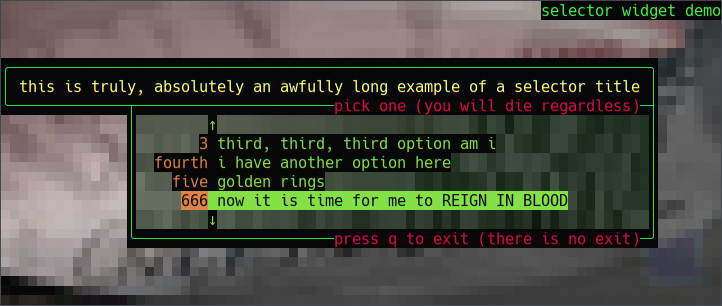
\includegraphics[width=.75\linewidth]{media/selector1.png}
    \caption{Selector with a long title.}
\end{figure}

\begin{figure}
    \centering
    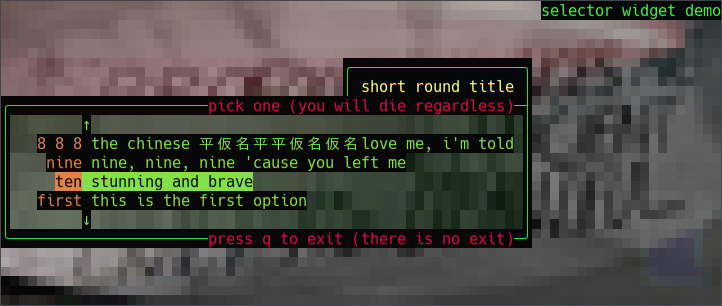
\includegraphics[width=.75\linewidth]{media/selector2.png}
    \caption{Short title intersecting with header.}
\end{figure}

\begin{figure}
  \centering 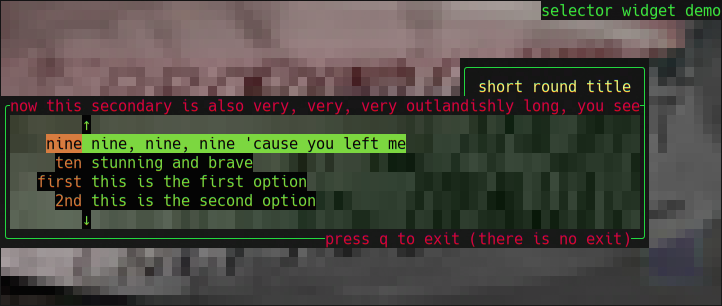
\includegraphics[width=.75\linewidth]{media/selector3.png}
    \caption{Selector with a long header.}
\end{figure}

\begin{figure}
\centering 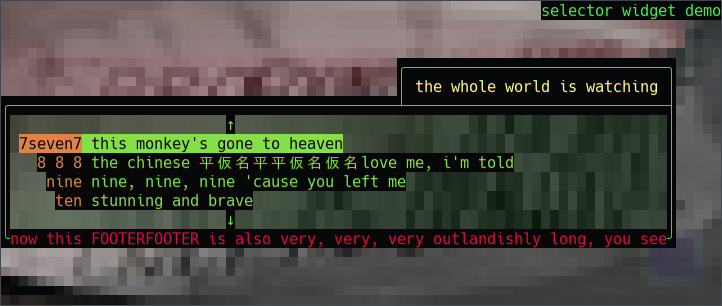
\includegraphics[width=.75\linewidth]{media/selector4.png}
\caption{Selector with a long footer and no header.}
\end{figure}

\begin{figure}
  \centering 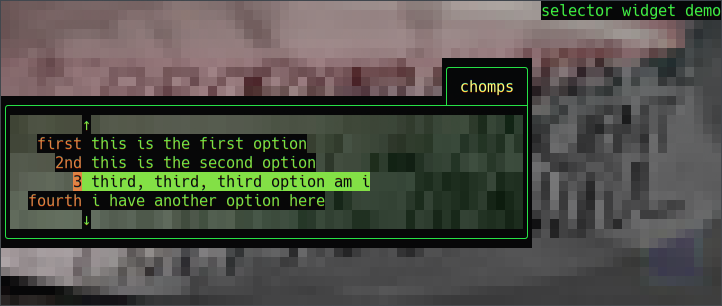
\includegraphics[width=.75\linewidth]{media/selector5.png}
  \caption{Naked selector.}
\end{figure}

\subsection{Menus}
\begin{figure}
    \centering
    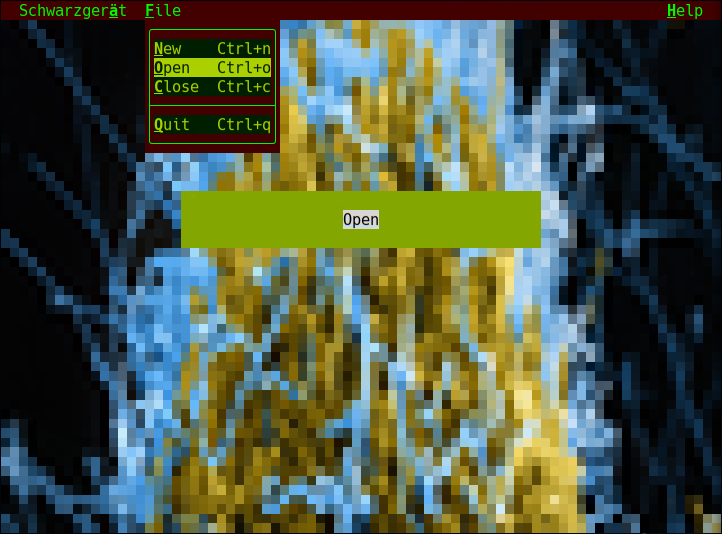
\includegraphics[width=.75\linewidth]{media/menutop.png}
    \caption{Menu along the top of the standard plane.}
\end{figure}

\begin{figure}
    \centering
    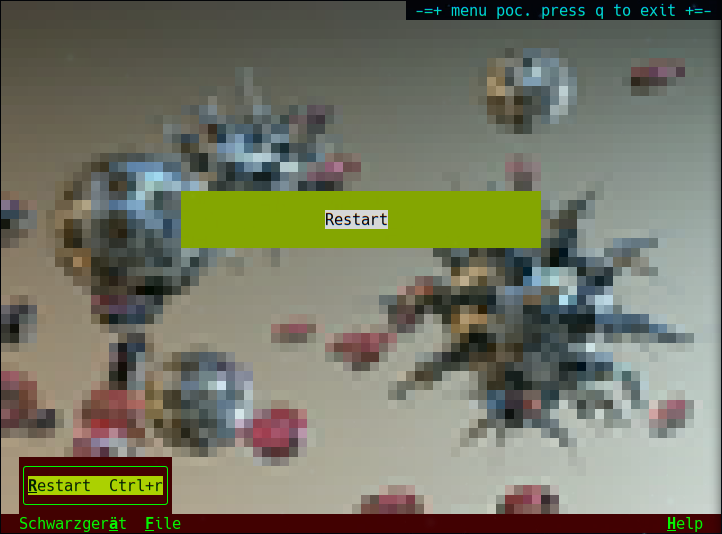
\includegraphics[width=.75\linewidth]{media/menubottom.png}
    \caption{Menu along the bottom of the standard plane.}
\end{figure}

\begin{figure}
    \centering
    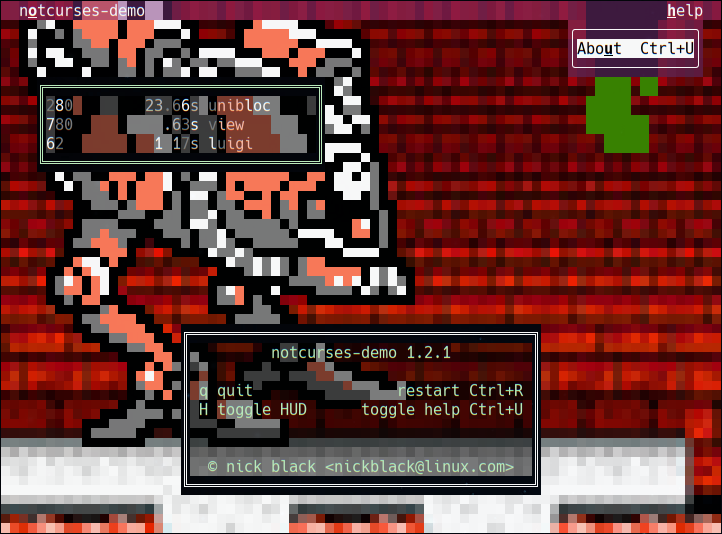
\includegraphics[width=.75\linewidth]{media/menuwarmech.png}
    \caption[WarMECH and a translucent menu.]{The \texttt{notcurses-demo} menu, unrolled \textit{in media res}. Luigi, pursued
      by WarMECH, is leaping through the ``Help'' menu. In the upper left is the HUD,
      and at the bottom the About text, both implemented as translucent planes.}
\end{figure}

\subsection{Reels}
\subsection{Example: let's rip off \texttt{whiptail}}

\section{Hack the Planet!}
\subsection{Example: let's rip off tetris}
\label{section:casestudy}
\subsection{Example: walking through \texttt{notcurses-demo}}
The \texttt{notcurses-demo} program is built as part of Notcurses, and ought
have been installed alongside the library (on Debian, you'll need the
\texttt{notcurses-bin} package, and even then the demo has been somewhat
reduced in order to comply with the DFSG\cite{dfsg}). It demonstrates a wide
range of Notcurses capabilities, and its source code is most instructive.

It is best to run the demo in a terminal having geometry of at least 80x45,
though anything 80x24 or larger will more or less work (some content will be
clipped). It is also desirable to have 24-bit color enabled, assuming your
terminal supports it. Determine the number of colors advertised by your
terminal type using~\texttt{infocmp} (see Figure~\ref{fig:terminfocmp}).
Some relevant terminfo capabilities are described in Table~\ref{table:terminfo}.

\begin{table}[h]
  \begin{center}
    \begin{tabular}{ |c|c|c| }
      \hline
      \texttt{colors} & Integer & Number of colors. \\
      \hline
      \texttt{ccc} & Boolean & The palette can be programmed. \\
      \hline
      \texttt{RGB} & Boolean & Direct RGB values can be speficied. \\
      \hline
    \end{tabular}
  \end{center}
  \caption{Relevant terminfo properties.}
  \label{table:terminfo}
\end{table}

Each demo makes use of a few different Notcurses capabilities. In addition,
a menu is present throughout. From this menu (or using keyboard shortcuts),
you can activate a HUD (H) and an informational help display (Ctrl+u). In
addition, you can restart the demo with Ctrl+R, or quit at any time (q). This
application serves admirably for benchmarking certain terminal behaviors, and
we'll do exactly that in Appendix~\ref{sec:termshade}. The performance
properties of various components are described at length therein.

\begin{figure}[h]
  \centering
  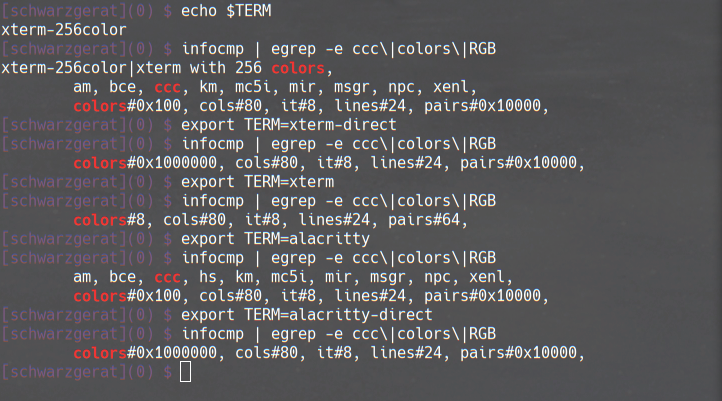
\includegraphics[width=.75\linewidth]{media/terminfocmp.png}
  \caption{Inspecting the terminfo database.}
  \label{fig:terminfocmp}
\end{figure}

Screenshots were taken using \texttt{scrot} 1.2 and a 80x45
\texttt{xfce4-terminal} 0.8.9.1 from Xfce 4.14+Compiz 0.8.16.1 atop Xorg
1.20.7 on NVIDIA 440.59. All of these are the unmodified Debian Unstable
x86\_64 binaries. My kernel is a custom 5.5.6 build. The terminal type is
\texttt{xterm-256color}, and \texttt{COLORTERM} is defined to be
\texttt{24bit}.

\newpage

\begin{figure}
  \centering
  \begin{minipage}{0.45\textwidth}
    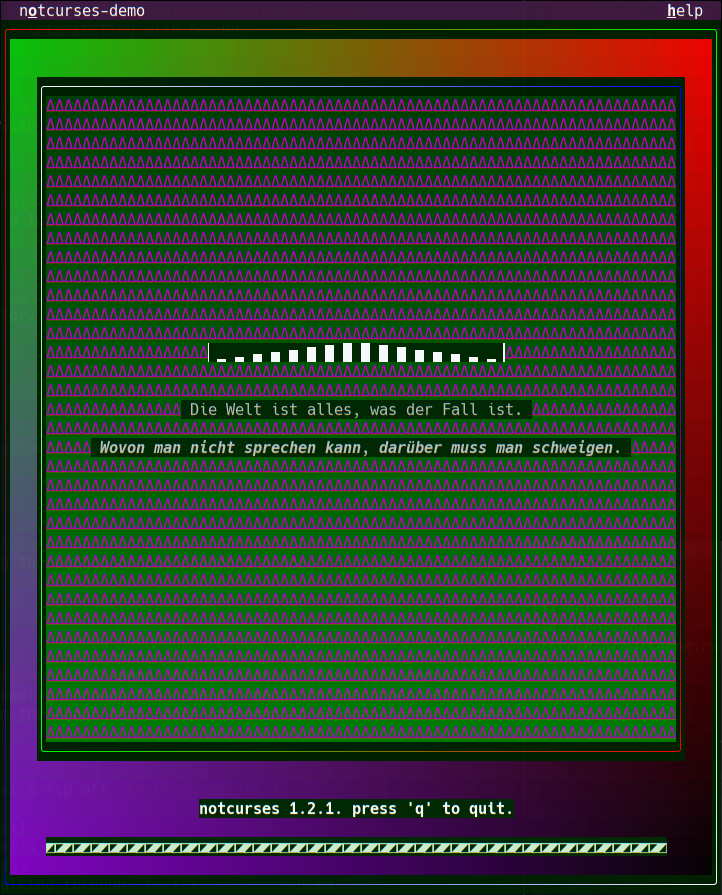
\includegraphics[width=1\linewidth]{media/demo-intro.png}
    \caption[``Intro''.]{``Intro''. Lerps on the perimeters. Inverse radial
            gradient plus vertical gradient. Full-screen fade.
            Cyclic glyphs. Italics.}
  \end{minipage}\hfill
  \begin{minipage}{0.45\textwidth}
    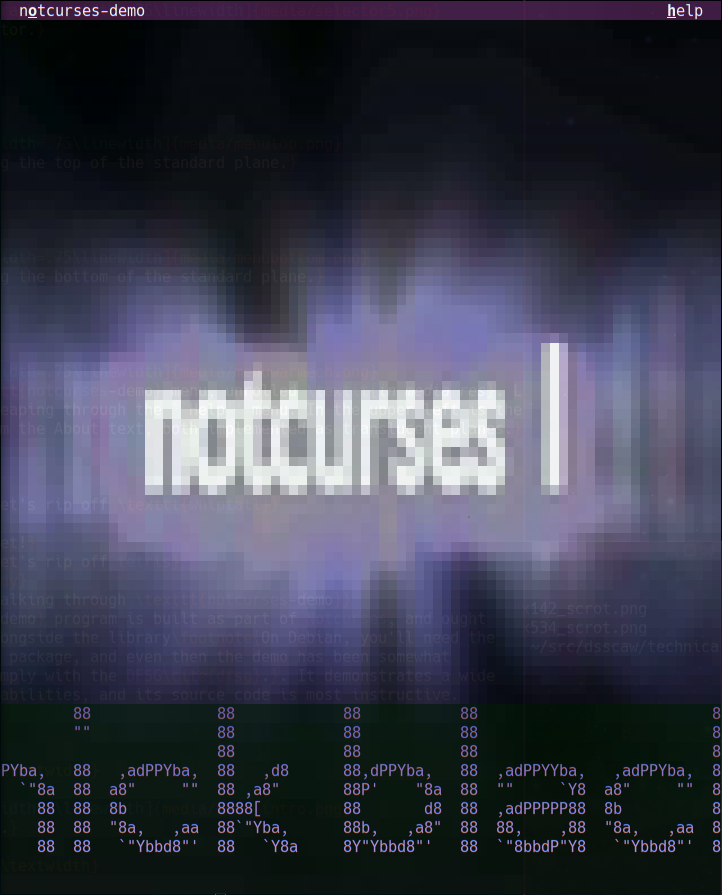
\includegraphics[width=1\linewidth]{media/demo-xray.png}
    \caption[``X-Ray''. Very large planes.]{``X-Ray''. Streaming video.
       Very large planes (the scrolling plane at the bottom is much larger than the visible screen).}
  \end{minipage}
\end{figure}

\begin{figure}
  \centering
  \begin{minipage}{0.45\textwidth}
    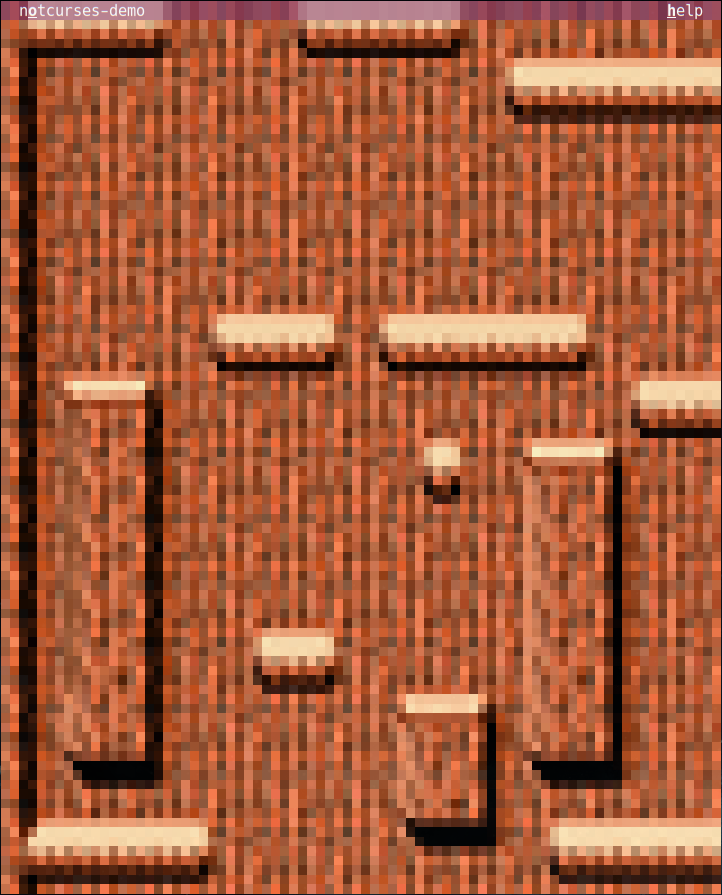
\includegraphics[width=1\linewidth]{media/demoeagle2.png}
    \caption{``Eagle'', first phase.\\
      Parallax scrolling on large image.}
  \end{minipage}\hfill
  \begin{minipage}{0.45\textwidth}
    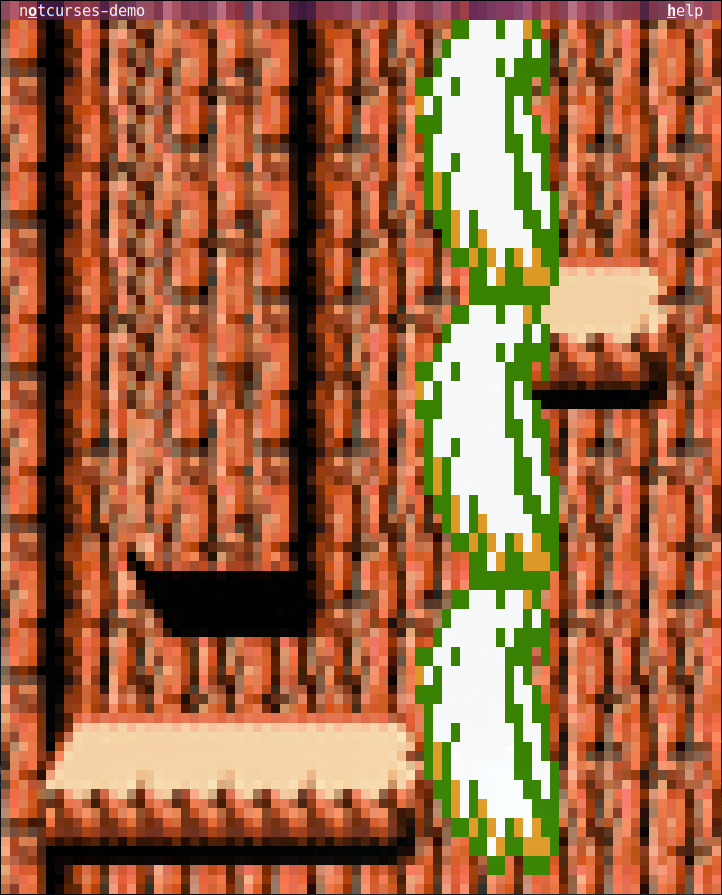
\includegraphics[width=1\linewidth]{media/demoeagle1.png}
    \caption{``Eagle'', second phase.\\
      Sprites. Zoomed image.}
  \end{minipage}
\end{figure}

\begin{figure}
  \centering
  \begin{minipage}{0.30\textwidth}
    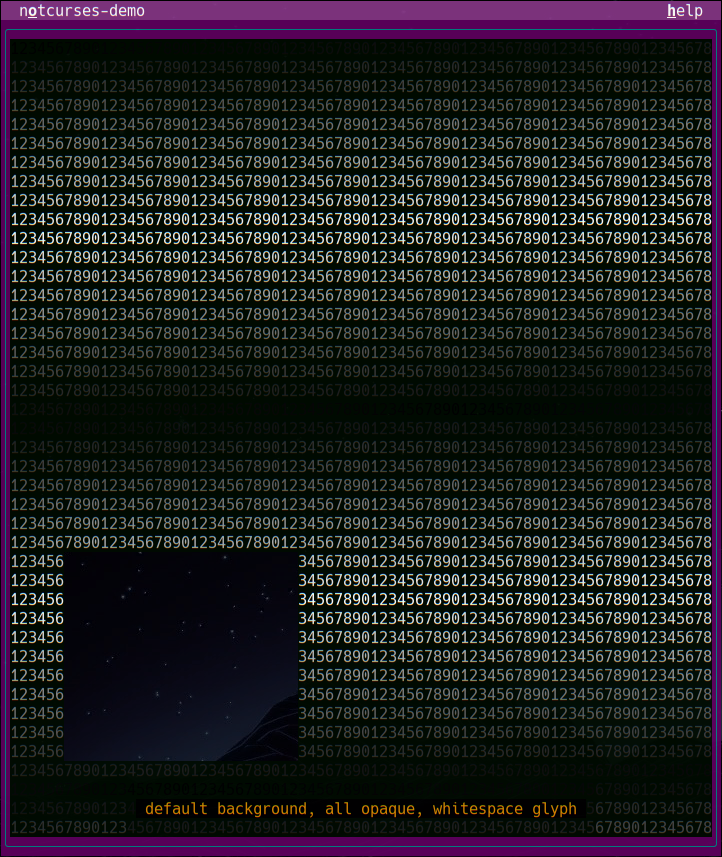
\includegraphics[width=1\linewidth]{media/demo-trans1.png}
    \caption[``Trans'', early phase.]{``Trans''. Transparent top plane. Window through to the desktop.}
  \end{minipage}\hfill
  \begin{minipage}{0.30\textwidth}
    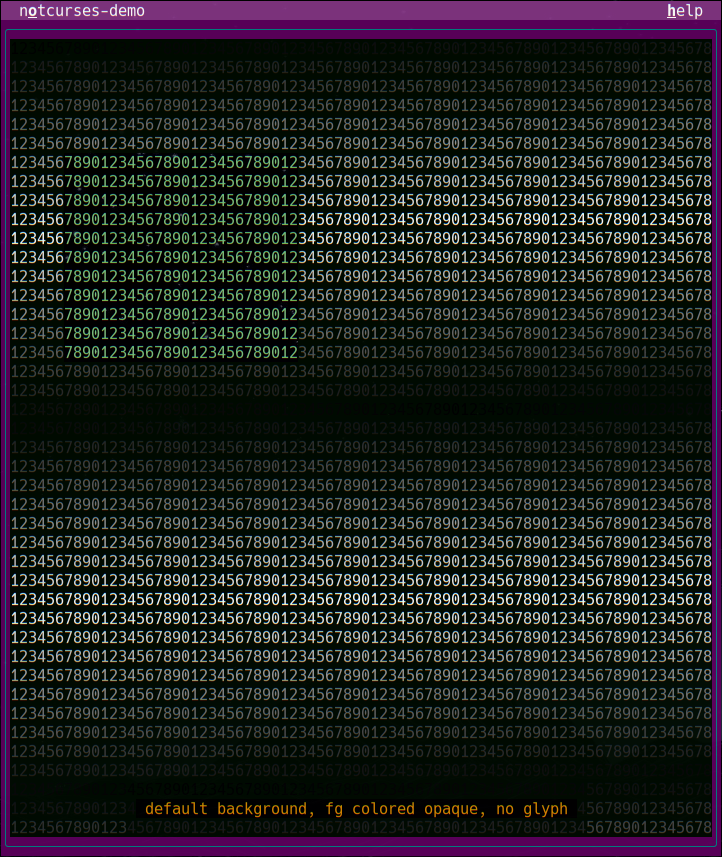
\includegraphics[width=1\linewidth]{media/demo-trans2.png}
    \caption[``Trans'', middle phase.]{``Trans''. Opaque foreground, transparent background, no glyph.}
  \end{minipage}\hfill
  \begin{minipage}{0.30\textwidth}
    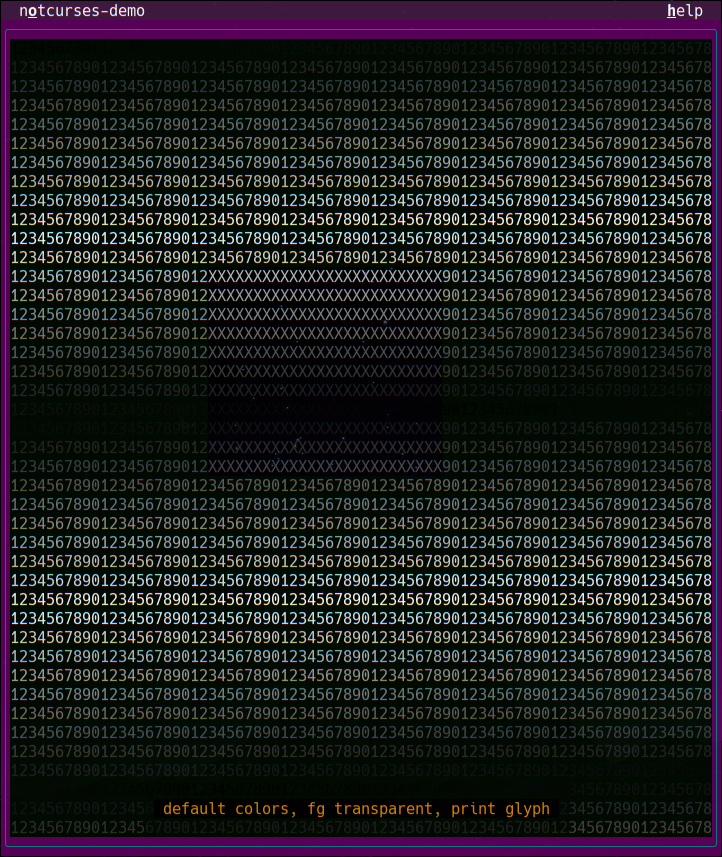
\includegraphics[width=1\linewidth]{media/demo-trans3.png}
    \caption[``Trans'', late phase.]{``Trans''. Transparent foreground and background with opaque glyph.}
  \end{minipage}\hfill
\end{figure}

\begin{figure}
  \centering
  \begin{minipage}{0.45\textwidth}
    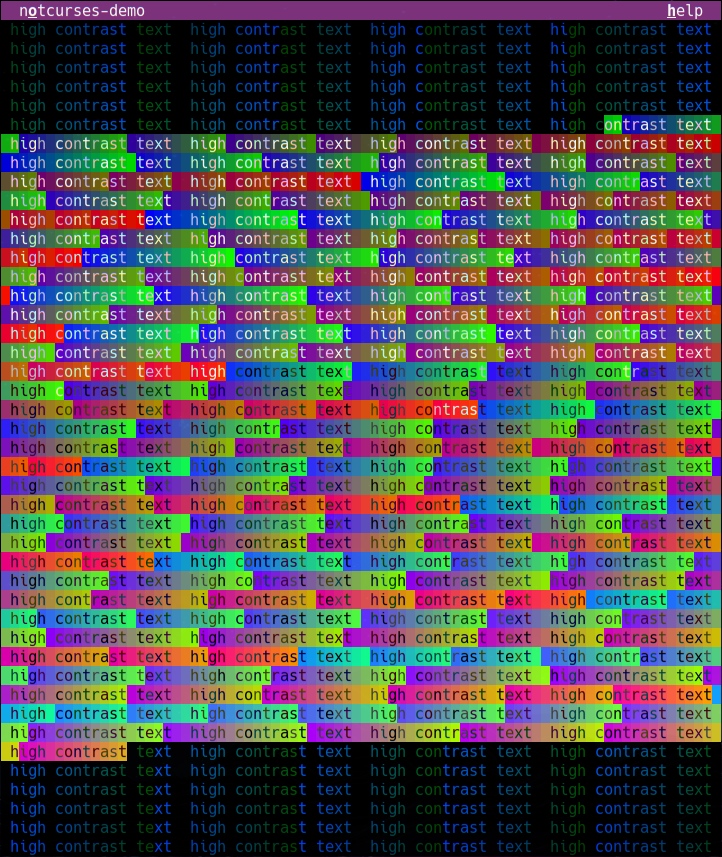
\includegraphics[width=1\linewidth]{media/demo-highcon.png}
    \caption{``Highcon''. High-contrast text.}
  \end{minipage}\hfill
  \begin{minipage}{0.45\textwidth}
    \includegraphics[width=1\linewidth]{media/demo-grid.png}
    \caption{``Grid''. Max RGB density.}
  \end{minipage}\hfill
\end{figure}

\begin{figure}
  \centering
  \begin{minipage}{0.45\textwidth}
    \includegraphics[width=1\linewidth]{media/demo-box.png}
    \caption{``Box''. Lerped perimeters. Precise Unicode. Color sweeps.}
  \end{minipage}\hfill
  \begin{minipage}{0.45\textwidth}
    \includegraphics[width=1\linewidth]{media/demo-sliders.png}
    \caption{``Sliders''. Partial fades. Animation. Gradients.}
  \end{minipage}\hfill
\end{figure}

\begin{figure}
  \centering
  \begin{minipage}{0.45\textwidth}
    \includegraphics[width=1\linewidth]{media/demo-reels.png}
    \caption{``Reels''. The \texttt{ncreel} widget.}
  \end{minipage}\hfill
  \begin{minipage}{0.45\textwidth}
    \includegraphics[width=1\linewidth]{media/demo-whiteout.png}
    \caption{``Whiteout''. Translucency.}
  \end{minipage}\hfill
\end{figure}

\begin{figure}
  \centering \includegraphics[width=.75\linewidth]{media/demo-chunli1.png}
  \caption{``Chunli''. Sprite animation.}
\end{figure}

\begin{figure}
  \centering \includegraphics[width=.75\linewidth]{media/demo-chunli2.png}
  \caption{``Chunli''. Sprite animation.}
\end{figure}

\begin{figure}
  \centering
  \begin{minipage}{0.45\textwidth}
    \includegraphics[width=1\linewidth]{media/demo-uniblock1.png}
    \caption{``Uniblock''. Hangul syllables.}
  \end{minipage}\hfill
  \begin{minipage}{0.45\textwidth}
    \includegraphics[width=1\linewidth]{media/demo-uniblock2.png}
    \caption{``Uniblock''. Emoji.}
  \end{minipage}\hfill
\end{figure}

\begin{figure}
  \centering
  \begin{minipage}{0.45\textwidth}
    \includegraphics[width=1\linewidth]{media/demo-img1.png}
    \caption{``View''. Scaling an image.}
  \end{minipage}\hfill
  \begin{minipage}{0.45\textwidth}
    \includegraphics[width=1\linewidth]{media/demo-img2.png}
    \caption{``View''. Transparent images.}
  \end{minipage}\hfill
\end{figure}

\begin{figure}
  \centering
  \begin{minipage}{0.45\textwidth}
    \includegraphics[width=1\linewidth]{media/demo-view1.png}
    \caption{``View''. Streaming video with high-contrast text.}
  \end{minipage}\hfill
  \begin{minipage}{0.45\textwidth}
    \includegraphics[width=1\linewidth]{media/demo-view2.png}
    \caption{``View''. Notice the high-contrast kicking in.}
  \end{minipage}\hfill
\end{figure}

\begin{figure}
  \centering \includegraphics[width=1\linewidth]{media/demojungle.png}
  \caption[``Jungle''. Palette-indexed image.]{``Jungle''. Palette-indexed image. Very low-bandwidth animation via palette cycling.\\
    ``Ruins in Rain'' © Mark Ferrari/Living Worlds. Texelized with permission.}
\end{figure}


\begin{figure}
  \centering
  \begin{minipage}{0.45\textwidth}
    \includegraphics[width=1\linewidth]{media/demo-fallin1.png}
    \caption[``Fallin\''', early phase.]{``Fallin\'''. Color change, introspection, many planes.}
  \end{minipage}\hfill
  \begin{minipage}{0.45\textwidth}
    \includegraphics[width=1\linewidth]{media/demo-fallin2.png}
    \caption[``Fallin\''', late phase.]{``Fallin\'''. The underlying image is revealed.}
  \end{minipage}\hfill
\end{figure}

\begin{figure}
  \centering
  \begin{minipage}{0.45\textwidth}
    \includegraphics[width=1\linewidth]{media/demo-luigi.png}
    \caption{``Luigi''. Multiple sprites.}
  \end{minipage}\hfill
  \begin{minipage}{0.45\textwidth}
    \includegraphics[width=1\linewidth]{media/demo-outro.png}
    \caption{``Outro''. Fades atop video.}
  \end{minipage}\hfill
\end{figure}

\newpage
%%%%%%%%%%%%%%%%%%%%%%%%%%%%%%%%%%%%%%%%%%%%%%%%%%%%%%%%%%%%%%%%%%%%%%%%

\begin{appendices}
\section{A brief history of character graphics}
\label{sec:terminals}
The earliest terminals making use of glyphs\footnote{Konrad Zuse's Z3, generally
 considered the first programmable digital computer, communicated with its
operator through a matrix of blinkenlights and a not unsteampunkish keyboard that resembled the
Burroughs typewriters of its era\cite{zuse}.} printed them to paper, and are of
interest to us only so far as our modern term ``tty'' is rather dubiously
derived from ``TeleTYpewriter'', as these cantankerous contraptions were
known\footnote{Though we do hear of their Snoopy calendars in the songs of
legend\cite{quiche}.} (people had less experience abbreviating in those days).

These devices most typically printed 72 characters per line (CPL), a limit that
has persisted in strange places\cite{pandoc} through the modern era. Another constant
you'll see from time to time is 132 CPL, derived from line printers such as the
IBM 1403, the DEC LP11, and the Centronics 101\cite{ibm1403}. Most often,
however, is the 80 column line originating in 1928's 7¾x3¼x0.007in IBM
Computer Card (as designed by Clair D.\ Lake, deriving from the 1890 U.\ S.\
Census cards of Herman Hollerith\ldots themselves borrowing from Joseph
Jacquard's automation in 1804 of punched card loom control technology pioneered
by Basile Bouchon in 1725\cite{cards}). To this day, so long as your wacky
output device can do 80 columns, eh, that's good enough. In all these cases,
the limit arises from the number of characters that could be printed, using the
technology of the time, on their feeder paper (8.5in and 14in in the case of
printers).

On, then, to the ``Glass TTYs'' (ugh) and Visual Display Units of the 1970s.
Pictured are the Computer Terminal Corporation Datapoint 3300, the
Lear Sigler, Inc.\ ADM-3A, the Hazeltine 1500, and the Soroc IQ-120~\ref{fig:terminals}.
Lacking microcontrollers, and generally implementing no independent control
sequences, such devices are today often known as ``dumb terminals'' (this term
was originally a registered trademark of Lear Sigler, see below). Already the
80x24 ``standard'' (it is not a standard) was emerging (the DEC contemporaries
listed were already pretty ``smart'', using proprietary control codes):

\begin{table}[h]
\begin{center}
  \begin{tabular}{ |c|c|c| }
    \hline
    IBM 2260 Model 1 & 1965 & 40x6 \\
    \hline
    Datapoint 3300 & 1969 & 72x25 \\
    \hline
    DEC VT05 & 1970 & 72x24 \\
    \hline
    IBM 3277 Model 2 & 1971 & 80x24 \\
    \hline
    Textronix 4010 & 1972 & 74x35 \\
    \hline
    DECscope VT52 & 1974 & 80x24 \\
    \hline
    LSI ADM-3A & 1976 & 80x12, 80x24 \\
    \hline
    Hazeltine 1500 & 1977 & 80x24 \\
    \hline
    Sororc IQ-120 & 1977 & 80x24 \\
    \hline
  \end{tabular}
\caption{Some historical terminals and their resolutions.}
\end{center}
\end{table}

Why 80x24 (or 80x25, as you'll also see)\cite{infoworld80}? The 80 almost certainly arises from
the desire to display an entire punched card (this \textit{is} a standard---see
ANSI X3.21-1967/FIPS PUB 13, ``Rectangular Holes in Twelve-Row Punched
Cards'')\cite{sonicdelay}. The origin of 24 is less clear. 24 is highly
composite (it has more divisors than any smaller number), and it is the largest
integer divisible by all natural numbers not larger than its square root. There
are of course 24 hours in a day. 24 divides the scanline counts of both NTSC
and PAL at 480 and 576, respectively. 24 rows of 80 columns at a byte per
column utilize 93.75\% of a 2KiB memory, leaving exactly 128 bytes left over,
and everyone loves a good power of 2.

The Aaronites, Levite descendents of Moses's brother Aaron, the first
\texthebrew{כהן גדול}
(High Priest),
form the priestly \texthebrew{כֹּהֲנִים}; they were divided into 24 courses. The Buddha's Dharma Chakra (Wheel of Dhamma)
in its Ashoka form extends 24 spokes. But perhaps I grow esoteric, and even
speculative\ldots in truth, 80x24 almost certainly owes its questionable
existence to IBM's punched cards, IBM 2260 and 3270 wanting compatibility with
IBM printers, the upstart DEC wanting compatibility with IBM software for their
VT52 and legendary VT100, and the VT100 subsequently becoming a \textit{de facto} standard for
four decades.

\begin{figure}
  \centering \includegraphics[width=.9\linewidth]{media/dumbterminals.jpg}
\caption[Dumb terminals of the 1970s.]{Clockwise starting from upper left: a dork and his LSI ADM (``American
  Dream Machine'', supposedly). That poor woman with the Sororc IQs looks stoned out
  of her gourd. Grizzly Adams rocks a Datapoint 3300, but really his mind is on
  seeing Skynyrd shred it this weekend. Finally, we have Frank the Cocaine
  Ranger and his Electric Hazeltine 1500 Band. \textit{Gott im Himmel}, the 70s were \textit{unseemly}.}
\label{fig:terminals}
\end{figure}

\begin{figure}
  \begin{minipage}{0.5\textwidth}
  \centering
    \includegraphics[width=.5\linewidth]{media/digital-terms.jpeg}
    \caption{Digital Equipment Corporation terminals of the 1970s and 1980s.}
  \end{minipage}\hfill
  \begin{minipage}{0.4\textwidth}
  \centering
    \includegraphics[width=.45\linewidth]{media/vt220-charset.png}
    \caption[VT220 glyph dump.]{The VT220's glyphs from a ROM dump. VT100 implemented most of the
      first seven columns. Note the existence of box-drawing characters\cite{crttypography}.}
  \end{minipage}\hfill
\end{figure}

\subsection{The DEC VTxxx terminals and ANSI X3.64-1979}

Introduced in August 1978, the VT100 ushered in a new era of smart terminals
using commodity (Intel) microprocessors, implementing portions of the upcoming
ANSI X3.64 standard (itself based on 1976's first edition of ECMA-48) along
with DEC extensions\footnote{The VT100 \textit{did not} implement all of X3.64,
nor was X3.64 derived from the VT100. The VT100 didn't do color, nor did it
insert or delete lines. It furthermore implemented several features outside
the scope of ECMA-48's first edition.} This series would go on to sell over
six million units, and it was a rare vendor that didn't include some degree
of DEC VT compatibility. Each major iteration of the series was designed to
encompass all functionality of prior iterations, beginning with the VT100's
faithful emulation of the earlier era's VT52. The VT102 cut down on the cost
and size of the VT100, and included the 132-CPL mode by default; they were
otherwise essentially the same device\cite{vt100}.

The original \texttt{xterm} was written as an emulator of the VAXStation 100
(VS100), and slowly acquired scattered features from the VT100, ANSI, and other
sources\cite{xtermfaq}. Thomas E.\ Dickey (the current maintainer of \Gls{ncurses}
and xterm) began working on XTerm in the mid-90s, and by 1996 had added the
\texttt{decTerminalID} resource following the addition of much VT220 compatibility.

\textbf{FIXME keep goin'\ldots}

\subsection{The Curses API}

\newpage
%%%%%%%%%%%%%%%%%%%%%%%%%%%%%%%%%%%%%%%%%%%%%%%%%%%%%%%%%%%%%%%%%%%
\section{Wherein I throw shade at current terminal emulators}
\label{sec:termshade}
\textbf{FIXME FIXME FIXME}
graphs i want:
\begin{denseitemize}
\item{emulator performance as a function of size}
\item{emulator performance as a function of bandwidth--same color everywhere, but turn off elision}
\item{emulator performance as a function of color change--difference with color restored relative to previous}
\item{emulator performance as a function of glyph variation}
\item{some basic perf flame graphs}
\end{denseitemize}
\newpage
%%%%%%%%%%%%%%%%%%%%%%%%%%%%%%%%%%%%%%%%%%%%%%%%%%%%%%%%%%%%%%%%%%%

\section{The Linux console}
The Linux console\footnote{The FreeBSD console is its own bag of wonders.} is
substantially different from the X and Wayland terminal emulators to which one
might be more accustomed\footnote{Muddying the issue is the fact that video
backends are sometimes described as consoles. The ``Linux console'' is a terminal
emulator running atop some video backend---on the x86, typically either VGA
Text Mode, or some trivial renderer atop a graphics-mode framebuffer
(e.\ g.\ EFIfb or vesafb.}. Modern terminal emulators are generally more capable
than the Linux console in several ways:

\begin{denseitemize}
\item{While the Linux console accepts RGB specifiers, it downsamples them to
    far fewer colors.}
\item{Console font capabilities are extremely limited.}
\end{denseitemize}

Like any interface to a termios\cite{termios} implementation, the \texttt{IUTF8}
flag should be set (consult \texttt{stty}). This can be accomplished with the
\texttt{IUTF8} termios flag (or \texttt{stty iutf8} on the command line). This
is necessary for the terminal to interpret your output as multibyte UTF-8. The
keyboard driver ought be placed into UTF-8 mode using the \texttt{KDSKBMODE}
ioctl; the \texttt{kbd-mode} tool does this when invoked with \texttt{-u}.
This is necessary for character erase to function properly in cooked mode. Some
keyboards generate scancodes beyond the essential 128 characters, and these
should be mapped to their UTF-8 equivalents. This can be accomplished with
\texttt{dumpkeys | loadkeys --unicode}\footnote{If you've ever seen the script
\texttt{unicode\_start}, this is exactly what it does.}. This functionality has
been supported since Linux 2.6.4, released 2004-03-11, and is almost certainly
already being done in your environment.

Ensure, as always, that \texttt{LANG} is properly set, that your program
initializes the locale with \texttt{setlocale(3)}, and that \texttt{TERM} is
properly set (in this case, to one of the ``linux*'' variants).

\textbf{FIXME FIXME FIXME talk about console font}

Consult the \textit{The Linux Programmer's Manual} for more information,
particularly
\texttt{ioctl\_console(2)}\cite{ioctlconsole},
\texttt{ioctl\_tty(2)}\cite{ioctltty},
\texttt{termios(3)}\cite{termios},
\texttt{console\_codes(4)}\cite{consolecodes},
and
\texttt{charsets(7)}\cite{charsets7}.

\newpage
%%%%%%%%%%%%%%%%%%%%%%%%%%%%%%%%%%%%%%%%%%%%%%%%%%%%%%%%%%%%%%%%%%%
\section{Unicode 13}
The Unicode Consortium has scheduled Unicode 13.0 for a March 2020 release.
Chapters 3 and most of Chapter 4 of the Core Specification are normative. The
remainder is informative. The Unicode Standard consists of the Core
Specification\cite{unicode13}, the \href{https://www.unicode.org/charts/}{code charts},
the \href{https://unicode.org/versions/Unicode13.0.0/#Unicode_Standard_Annexes_nb}{Unicode Standard Annexes}
, and the \href{http://www.unicode.org/Public/13.0.0/}{Unicode Character Database (UCD)}.

\begin{table}[h]
\begin{center}
  \begin{tabular}{ |c|c| }
    \hline
    UAX \#9 & Unicode Bidirectional Algorithm \\
    \hline
    UAX \#11 & East Asian Width \\
    \hline
    UAX \#14 & Unicode Line Breaking Algorithm \\
    \hline
    UAX \#15 & Unicode Normalization Forms \\
    \hline
    UAX \#24 & Unicode Script Property \\
    \hline
    UAX \#29 & Unicode Text Segmentation \\
    \hline
    UAX \#31 & Unicode Identifier and Pattern Syntax \\
    \hline
    UAX \#34 & Unicode Named Character Sequences \\
    \hline
    UAX \#38 & Unicode Han Database (Unihan) \\
    \hline
    UAX \#41 & Common References for Unicode Standard Annexes \\
    \hline
    UAX \#42 & Unicode Character Database in XML \\
    \hline
    UAX \#44 & Unicode Character Database \\
    \hline
    UAX \#45 & U-Source Ideographs \\
    \hline
    UAX \#50 & Unicode Vertical Text Layout \\
    \hline
  \end{tabular}
\caption{Unicode 13.0.0 Standard Annexes.}
\end{center}
\end{table}

\begin{table}[h]
\begin{center}
  \begin{tabular}{ |c|c| }
    \hline
    UTS \#10 & Unicode Collation Algorithm \\
    \hline
    UTS \#39 & Unicode Security Mechanisms \\
    \hline
    UTS \#46 & Unicode IDNA Compatibility Processing \\
    \hline
    UTS \#51 & Unicode Emoji \\
    \hline
  \end{tabular}
\caption{Unicode 13.0.0 Synchronized Technical Standards.}
\end{center}
\end{table}

\newpage
%%%%%%%%%%%%%%%%%%%%%%%%%%%%%%%%%%%%%%%%%%%%%%%%%%%%%%%%%%%%%%%%%%%

\section{Notcurses header files}
\subsection{The \texttt{notcurses.h} header}
\bgroup
\inputminted[linenos,breaklines=true]{C}{code/notcurses.h}
\egroup

\subsection{The \texttt{nckeys.h} header}
\bgroup
\inputminted[linenos,breaklines=true]{C}{code/nckeys.h}
\egroup

\end{appendices}
\newpage
%%%%%%%%%%%%%%%%%%%%%%%%%%%%%%%%%%%%%%%%%%%%%%%%%%%%%%%%%%%%%%%%%%%%%%%%
\glsaddallunused
\printglossary[title={Glossary of terms}]
\newpage
%%%%%%%%%%%%%%%%%%%%%%%%%%%%%%%%%%%%%%%%%%%%%%%%%%%%%%%%%%%%%%%%%%%%%%%%
\addcontentsline{toc}{section}{References}
\printbibliography
%%%%%%%%%%%%%%%%%%%%%%%%%%%%%%%%%%%%%%%%%%%%%%%%%%%%%%%%%%%%%%%%%%%%%%%%
%\newpage
%\vfill
%\begin{center}
%\includegraphics[width=.4\linewidth]{../common/dsscaw-purp-scaled.png}
%\includegraphics[width=.5\linewidth]{../common/south.png}
%\end{center}
%\vfill
\end{document}
